\DocumentMetadata{lang=en-US}
\pdfinfoomitdate=1
\pdftrailerid{}
\pdfsuppressptexinfo=15
\pdfgentounicode=1
\documentclass[11pt]{article}
\usepackage[genericmode]{tagpdf}
\tagpdfsetup{activate-tree,activate-struct,tagunmarked}
\usepackage[margin=1in]{geometry}
\usepackage[T1]{fontenc}
\usepackage{lmodern}
\usepackage{amsmath,amssymb,amsthm}
\usepackage{booktabs,array,longtable,xcolor}
\usepackage{listings}
\usepackage{graphicx}
\usepackage{caption}
\captionsetup{font=small,labelfont=bf}
\usepackage[section]{placeins}
\usepackage{microtype}
\usepackage{xurl}
\usepackage{enumitem}
\usepackage[authoryear,round]{natbib}
\usepackage{hyperref}
\setcounter{tocdepth}{2}
\renewcommand{\bibsection}{\section*{\refname}\addcontentsline{toc}{section}{\refname}}
\hypersetup{
  colorlinks,
  linkcolor=blue!50!black,
  citecolor=blue!50!black,
  urlcolor=blue!50!black,
  pdftitle={Foundations of Formal Market Microstructure in U.S. Equities},
  pdfauthor={Miquel Noguer i Alonso},
  pdfsubject={Machine-checked allocation, composition, and necessary state for U.S. equity market mechanisms},
  pdfkeywords={Market microstructure, U.S. equities, formal verification, Lean 4, price-time priority, parity allocation, stream consistency, state identifiability},
  pdflang={en-US}
}
\lstset{basicstyle=\ttfamily\footnotesize,columns=fullflexible,keepspaces=true,breaklines=true}
\setlength{\emergencystretch}{3em}
\raggedbottom
\newtheorem{theorem}{Theorem}[section]
\newtheorem{proposition}[theorem]{Proposition}
\newtheorem{lemma}[theorem]{Lemma}
\newtheorem{corollary}[theorem]{Corollary}
\newtheorem{auditlemma}[theorem]{Audit lemma}
\theoremstyle{definition}
\newtheorem{definition}[theorem]{Definition}
\newtheorem{axiom}[theorem]{Axiom}
\newtheorem{example}[theorem]{Example}
\newtheorem{principle}[theorem]{Principle}
\theoremstyle{remark}
\newtheorem{remark}[theorem]{Remark}
\newcommand{\codeunderscore}{\char`\_\allowbreak}
\newcommand{\lean}[1]{\ifmmode\mathtt{#1}\else{\ttfamily\let\_\codeunderscore #1}\fi}
\newcommand{\N}{\mathbb{N}}
\newcommand{\Z}{\mathbb{Z}}
\newcommand{\NBB}{\mathrm{NBB}}
\newcommand{\NBO}{\mathrm{NBO}}
\newcommand{\tot}{\operatorname{tot}}
\newcommand{\plain}[1]{\par\smallskip\noindent\textcolor{blue!50!black}{\textbf{Plain-language reading.}} #1\par\smallskip}

\title{Foundations of Formal Market Microstructure\\
\Large in U.S. Equities\\[4pt]
\large Machine-Checked Allocation, Composition,\\ Necessary State, and Regulatory Traceability}
\author{Miquel Noguer i Alonso\\ Artificial Intelligence Finance Institute}
\date{September 5, 2026\\[4pt]
\small DOI: \href{https://doi.org/10.5281/zenodo.22343804}{10.5281/zenodo.22343804}\\[4pt]
\small GitHub: \href{https://github.com/MiquelNoguerAlonso/Formal-Verification}{MiquelNoguerAlonso/Formal-Verification}}

\begin{document}
\maketitle

\begin{abstract}
This paper develops executable models of price--time priority and parity allocation in U.S. equities to establish when execution consistency holds and which state must be retained. Splitting an order can change who receives shares. In a parity wheel, resetting the rotation between executions can alter allocations even when total incoming quantity is unchanged.

A counterexample shows that restarting the wheel between executions can change allocations. Preserving its participant pointer and unfinished lot allowance restores consistency between split and combined quantities on reachable states, under a positive lot size and an admissible first quantity. A further invariant recovers the unused allowance from the cumulative allocation of the current participant. Consequently, when the pointer and aligned cumulative fills are known, the allowance need not be stored independently.

The information results distinguish prediction from reconstruction. On specified nondegenerate families sharing an authenticated observation, every summary sufficient to predict future fills must distinguish live pointer positions. The pointer is sufficient once the family is fixed, and a reachable family attains the exact state bound. Separate finite families characterize the additional information required when cumulative fills are unavailable.

Supporting results establish allocation feasibility, conservation, priority, one-lot balance, and explicit approximation bounds relating wheel allocations to constrained equal awards. They also yield a conventional analytic limit as lot size vanishes. A decidable price--time checker is characterized by feasibility and seriality, with conformance preserved under sequential execution.

Lean 4.22.0 checks 362 theorem declarations using its core library. Axiom dependencies are audited explicitly; the analytic limit is distinguished from the formalized results. A dated regulatory ledger links 58 selected provisions or identified source items to executable definitions and audit records. These mappings support inspection without proving legal interpretation, evidence authenticity, or equivalence to a production exchange. The resulting framework connects allocation mechanisms, persistent state, and reproducible conformance analysis.
\end{abstract}

\noindent\textbf{Keywords:} Market microstructure; U.S. equities; formal verification; Lean~4; price--time priority; parity allocation; stream consistency; state identifiability.

\clearpage
\pdfbookmark[1]{Contents}{table-of-contents}
\tableofcontents
\clearpage

\section{Introduction}

\subsection{The claim}
An exchange receives marketable quantity as a stream. If 200 shares arrive at once or as two consecutive orders of 100, with no intervening order-book changes, a stream-consistent allocation mechanism should reach the same final state after processing the same total quantity. Price--time has this property using residual claims alone. A parity wheel does not: if every execution restarts at the first participant, order segmentation changes who trades.

The paper's central contribution is a state-and-information result. First, an executable counterexample proves that reset rotation violates Moulin composition. Second, a wheel that persists its participant pointer and unfinished round-lot phase satisfies exact split-versus-combined consistency on every reachable state and every admissible first estate. Third, for any indexed nondegenerate family with the same authenticated observation, future sufficiency forces a summary to encode the pointer injectively, and the pointer is itself a sufficient code once the family is fixed. A reachable full-allowance family realizes the exact $m$-state bound. Finally, on every reachable live-head state, the unused allowance is $L-(A_p\bmod L)$. Consequently, when participant-aligned cumulative fills are available, the allowance is derived rather than separately stored and the pointer label is the remaining phase datum in the stated observation model.

Market microstructure theory studies the economic consequences of trading rules \citep{ohara1995market,parlour1998price,harris2003trading}. Here executable allocation operators are the primitive objects. The paper also isolates the fixed-order characterization of price--time, proves one-lot balance and approximation to constrained equal awards, derives a vanishing-lot continuum limit, and turns the price--time characterization into a deterministic conformance check. These results concern the specified mechanisms. Correspondence with institutional rule text remains a modelling claim, and real-world compliance remains an evidentiary claim.

The selected mechanics use integer shares, round lots, tick-constrained prices, rotation, minimum, comparison, and lexicographic maximization. Their finite invariants are proved by structural induction and exact arithmetic in Lean. The continuum-limit corollary is a conventional real-analysis deduction from the machine-checked finite error bound. The strategic propositions in Appendix~\ref{sec:strategic} concern best responses in contests, rent dissipation, dilution of a privileged slot, and routing by net cost under additional behavioral assumptions.

\subsection{What is built}
Section~\ref{sec:objects} fixes the primitive objects. Section~\ref{sec:ops} defines the three allocation operators. Section~\ref{sec:algebra} gives their algebra: sequential composition, conservation closure, benchmark naturality, relabeling equivariance of the persistent wheel, and monotonicity. Section~\ref{sec:axioms} states the allocation predicates and Section~\ref{sec:char} proves uniqueness (seriality is price--time), a one-lot balance guarantee for the wheel, incompatibility, and ladder uniqueness. Section~\ref{sec:structure} adds completeness, conservation, displayed precedence, and price priority across levels. Section~\ref{sec:rationing} separates estate composition, water-level composition, and state-transition composition, proves feasibility of the estate-indexed unit rule, isolates the reset-composition obstruction, and proves that the persistent pointer wheel is both balanced and stream-consistent under stated hypotheses. Sections~\ref{sec:cross}--\ref{sec:auction} give cross-market and auction kernels. Section~\ref{sec:obs} proves non-identifiability, general fiberwise pointer minimality, and exact predictive-summary bounds on reachable finite families, with separate contracts for observers who already know cumulative fills. Section~\ref{sec:conformance} turns price--time uniqueness into a complete, decidable and composition-safe check. Section~\ref{sec:rule-register} registers every analytic rule family. Section~\ref{sec:clauses} gives the regulatory audit contract; Appendix~\ref{app:clauses} contains the dated clause ledger, inspection profiles, and source pinpoints. Section~\ref{sec:scope} separates theorem, traceability, and production claims. Appendix~\ref{sec:strategic} isolates optional strategic inequalities and their additional behavioral assumptions.

\subsection{Proof system}
The executable mechanisms and named theorem contracts are formalized in Lean~4 \citep{demoura2021lean4} version 4.22.0 with the core library only---no Mathlib \citep{mathlib2020}---as sixteen proof/test modules (including the axiom-audit module) plus one command-line checker entry point. \lean{Conformance.lean} contains deterministic test harnesses; \lean{AllocationRecord.lean} is the checker entry point. Each formal result below is annotated with its Lean declaration; fixed-length bit-encoding consequences in Section~\ref{sec:obs} are identified explicitly as mathematical corollaries of checked injectivity. The package builds with \lean{lake build}; \lean{Check.lean} prints the axiom dependency of all 362 theorem declarations; \lean{lake exe allocation\_record} runs the checker on a supplied order-level queue and queue-aligned fill vector. The source has no \lean{noncomputable} declaration and no use of \lean{Classical.choose}; executable definitions therefore remain distinct from the 48 theorem proof terms whose audited dependencies include \lean{Classical.choice}. Appendix~A names those declarations and gives exact contracts for load-bearing results.

\subsection{How to read this paper without advanced prerequisites}
No programming or proof-theory background is required to understand the economic claims. The formal notation makes each rule precise, but the central objects have direct market meanings.

\paragraph{The market picture.} A \emph{resting order} is an instruction already waiting at a venue. A new, marketable order arrives with a quantity to buy or sell. An \emph{allocation rule} decides how much of that incoming quantity each resting order receives. The resulting executed amounts are \emph{fills}. A \emph{queue-aligned allocation record} associates those fills with the supplied resting-order positions; unlike a public trade report, it is privileged audit data. A \emph{queue} is the ordered list of resting order sizes at one price.

\paragraph{The notation.} $\N$ means the whole numbers $0,1,2,\ldots$. A list such as $Q=(200,300,500)$ describes three resting orders. If $x=600$ shares arrive, an allocation such as $A=(200,300,100)$ says that the first order receives 200 shares, the second 300, and the third 100. The symbol $\min\{a,b\}$ means ``whichever number is smaller,'' $\sum$ means ``add the entries,'' and $\lfloor z\rfloor$ means ``round down to a whole number.'' A function is just a rule that turns specified inputs into an output.

\paragraph{The formal-verification picture.} Lean is software that checks a proof one logical step at a time. A Lean theorem is not a simulation and not a statistical confidence statement: if its assumptions are satisfied, its conclusion follows exactly. The clause layer prevents a named provision from disappearing silently, but it cannot decide whether a venue supplied truthful evidence for a procedural field. Clause coverage, theorem validity, and real-world compliance are therefore three different claims.

\paragraph{How to read a theorem.} Read each result as ``under these conditions, this guarantee follows.'' Text in typewriter font, such as \lean{priceTime\_sum\_le}, is the name of the matching Lean declaration; it can be ignored on a first reading. Proof ideas explain why a result is true, while the full machine-checked proof is in the accompanying source. A counterexample proves that a broad claim cannot hold in general by exhibiting one valid case in which it fails.

\paragraph{Abbreviations.} NBBO is the national best bid and offer; NBB and NBO are its bid and offer components. SIP is a securities information processor; ISO is an intermarket sweep order; DMM is a designated market maker; SRO is a self-regulatory organization; ATS is an alternative trading system; LULD is the Limit Up--Limit Down Plan; NMS is the national market system; and Reg SHO is Regulation SHO.

\paragraph{A running example.} Suppose the queue is $(200,300,500)$ and 600 shares arrive. Price--time gives $(200,300,100)$ because it finishes earlier orders before later ones. A parity wheel with a 100-share round lot can give $(200,200,200)$ by visiting each participant repeatedly. Both allocate 600 shares without exceeding any resting order, but they express different ideas of priority and balance. Much of the paper formalizes that difference.

Figure~\ref{fig:allocation} shows the running example in queue order: both mechanisms clear the incoming quantity while leaving different residual claims.

\begin{figure}[tbp]
\centering
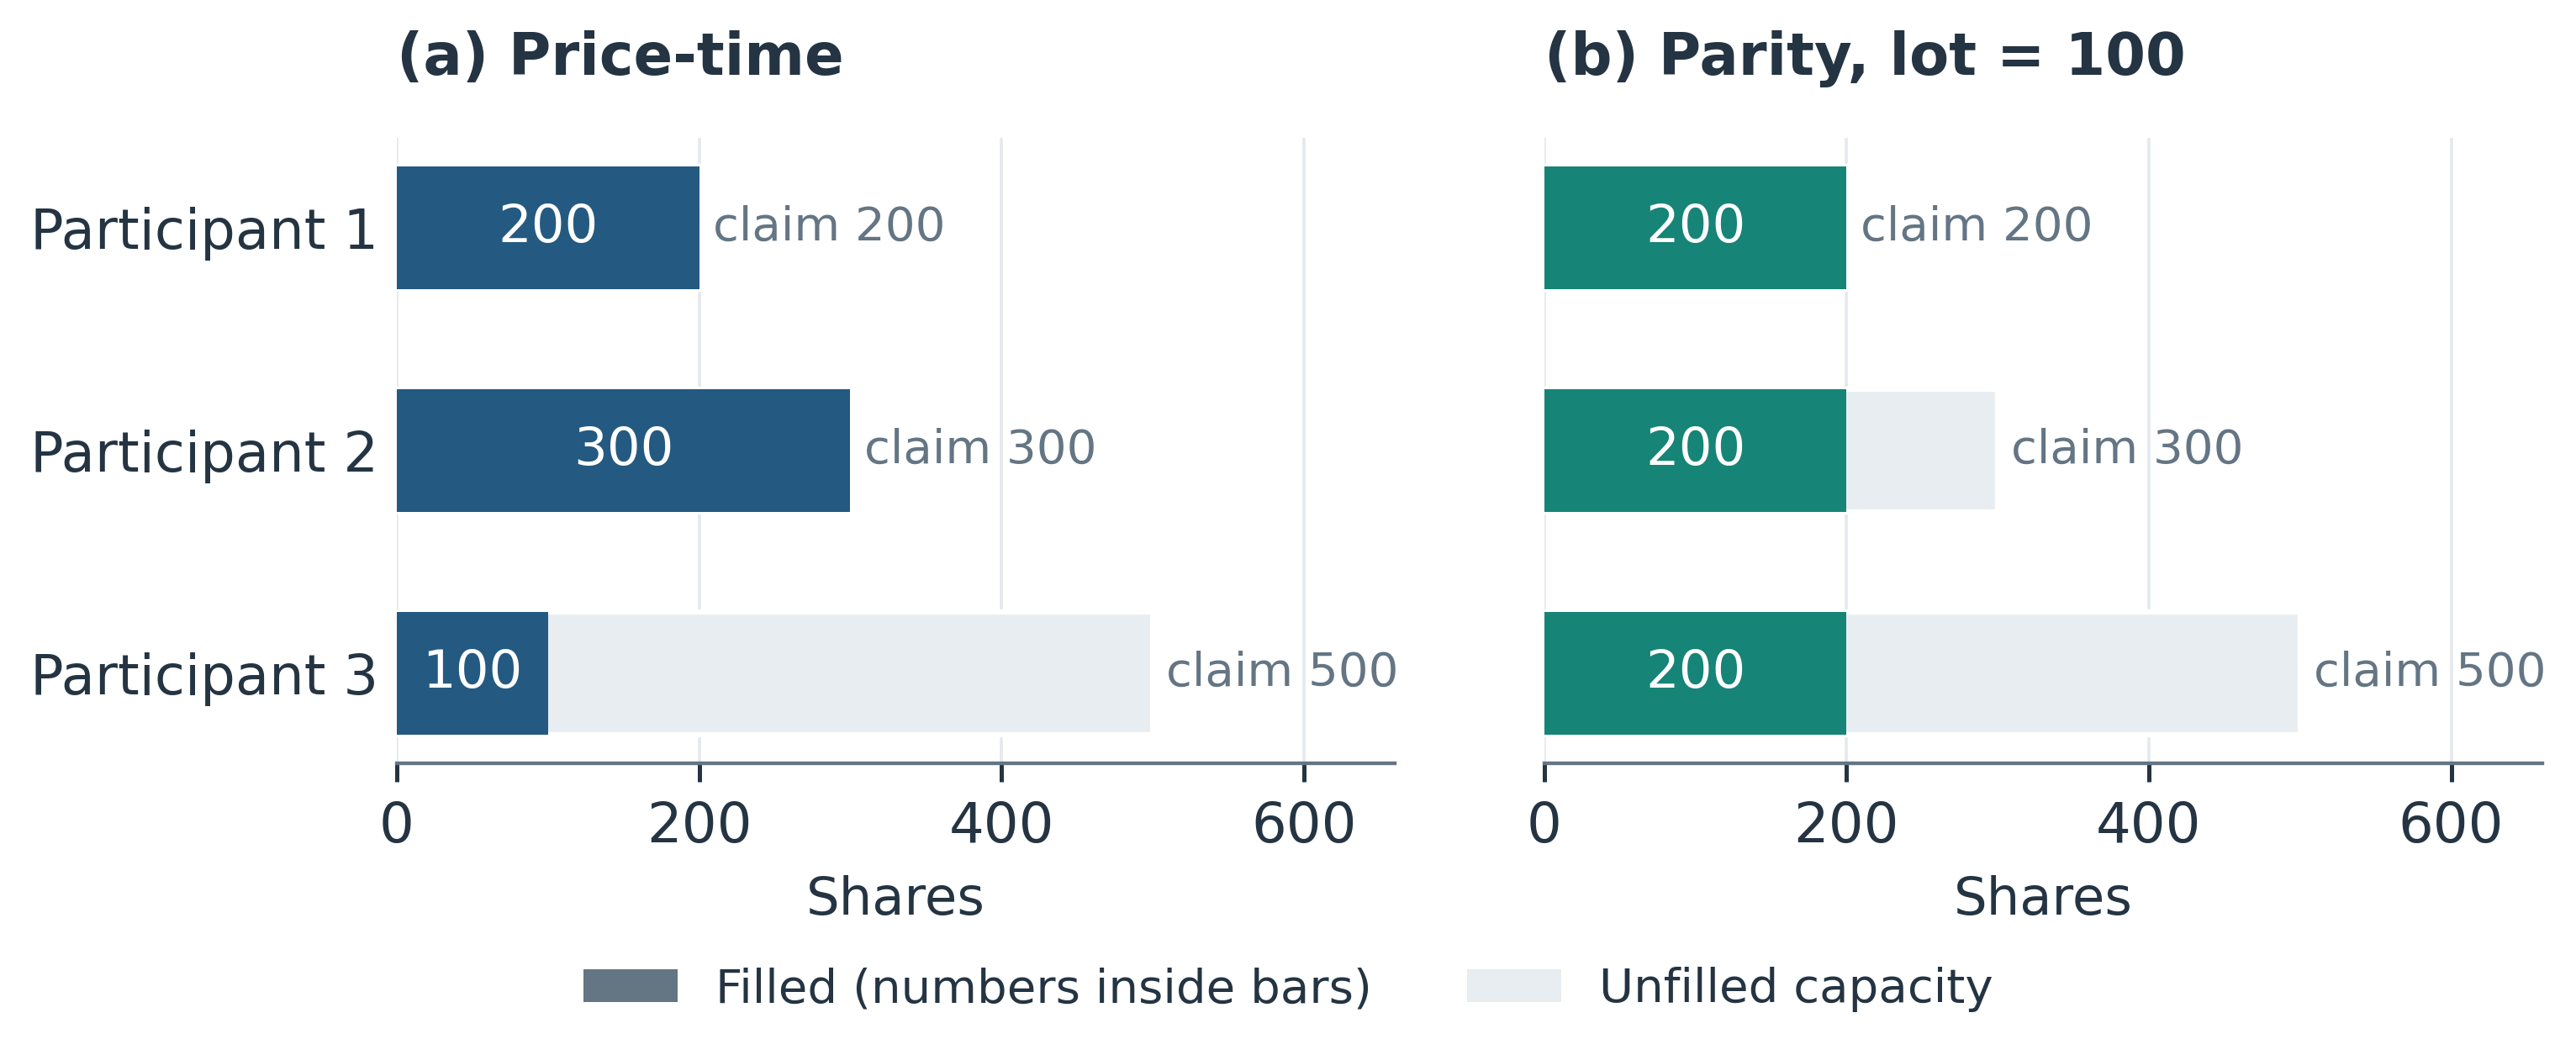
\includegraphics[width=\linewidth]{figures/allocation_comparison.png}
\caption{Price--time and parity on the same queue $Q=(200,300,500)$ with $x=600$. Colored segments are fills; the pale remainder is unfilled capacity. Price--time fills $(200,300,100)$, whereas the 100-share wheel fills $(200,200,200)$. Each row represents one participant, and both mechanisms allocate exactly 600 shares.}
\label{fig:allocation}
\end{figure}

\subsection{Related work}
Formal work on exchange mechanisms is directly relevant. \citet{sarswat2020} formalize fairness, uniformity, and individual rationality for financial-market trades; \citet{natarajan2021} extend verified double auctions to multiple quantities, prove uniqueness results, extract programs, and test them on market data; and \citet{garg2022} specify continuous double auctions, prove that three properties determine their input--output relation, and extract a verified trade-log checker. Verified financial software also includes the Imandra dark-pool analysis of \citet{passmore2017formal} and its later exchange digital-twin work \citep{brennan2024imandra}, as well as contract languages \citep{bahr2015certified}; formal law includes Catala \citep{merigoux2021catala}. The present contribution is narrower and complementary: machine-checked integer models of price--time allocation, NYSE-inspired setter/parity allocation, their rationing identities, and selected cross-market rule fragments. It does not claim the first formalization of exchange matching or automated conformance checking.

The round-robin structure of parity is related to fair queueing \citep{nagle1987fair}. The optional strategic layer connects to queue rationing under price controls \citep{yao2018tick}, fee structure \citep{comerton2019inverted}, fragmentation \citep{ohara2011fragmentation}, latency \citep{ding2014slow,bartlett2019latency}, frequent batch auctions \citep{budish2015hft}, and contest models \citep{tullock1980,baye1996allpay}. The axiomatic theory of rationing is due to \citet{young1987}, \citet{young1994}, and \citet{moulin2000}, and is surveyed by \citet{thomson2003}; \citet{aumann1985} provide the contested-garment lineage, \citet{herrero2001} study classical divisible rules, and \citet{herrero2008} study balanced claims allocation with indivisible units. The composition axiom is used here in the formulation emphasized by \citet{moulin2000}.

\section{Primitive objects}\label{sec:objects}

\begin{definition}[Quantities]
A share count is an element of $\N$. A round lot is a positive integer $L$. A price is an element of $\N$ in units of $\$0.0001$; we write $\lean{dollar}=10^4$, $\lean{penny}=100$.
\end{definition}

\begin{definition}[Queue]
A queue at a price is a finite participant-labelled list in a canonical external order:
\[
Q=((i_1,q_1),\dots,(i_m,q_m)).
\]
Serial allocation uses arrival order. The pointer-wheel state stores a rotated internal view whose head is the current pointer; statements about participant allocations compare outputs only after mapping that rotated view back to the canonical labels.
\end{definition}

\begin{definition}[Level, ladder]
A level is a price with a queue; on a hybrid venue it also carries a setter tranche $Q^{\mathrm s}$ (\lean{Level}). A ladder is a list of levels ordered by price.
\end{definition}

\begin{definition}[Participant state]
A participant is $(a,r)\in\N^2$: allocated so far, remaining. A level in state form is a list of participants; $a+r$ is invariant under allocation and equals the participant's original size.
\end{definition}

\begin{definition}[Quote]
A quote is (venue, price, size, automated) (\lean{Quote}). Within the model, it is protected iff automated and at least one round lot (\lean{protected\_}). Actual Regulation NMS protection also requires the quotation to be the exchange's best bid or offer; the model assumes its input has already been restricted to venue-top quotations \citep{sec2005regnms}.
\end{definition}

\begin{definition}[Fill, allocation record, market-data event]
A fill is an executed size. A queue-aligned allocation record is the vector of fills matched to the supplied order positions; it is an audit input and is not asserted to be a public tape. Separately, a market-data event carries a venue timestamp $v$ and a latency $\ell\ge0$ and is consolidated at $v+\ell$ (\lean{Ev}). The two-clock results concern only these timestamps, not participant-level attribution.
\end{definition}

\begin{definition}[Allocation, operator]
An allocation of $x$ over $Q$ is a list $A\in\N^m$. An operator is a function $x\mapsto(A,x')$ giving fills and leftover (\lean{Op}).
\end{definition}

For equal-length lists, write $A\oplus B:=\lean{List.zipWith (fun a b => a+b) A B}$ for componentwise addition and $Q\ominus A:=\lean{List.zipWith Nat.sub Q A}$ for residual claims. Here natural-number subtraction is truncated at zero. Every displayed sum of allocation vectors below uses $\oplus$.

Pointwise relations between lists of equal length are written with the inductive predicate $\lean{Pw}\,P$ (\lean{Pw.nil}, \lean{Pw.cons}).

\plain{The symbols summarize one transaction. $Q$ is what was available, $x$ is what arrived, $A$ is what traded against each resting order, and $x'$ is any quantity still unfilled. A correct rule must never fill more than was available and must account for every share.}

\section{The allocation operators}\label{sec:ops}

\begin{definition}[Serial: price--time; \lean{priceTime}]
$a_i=\min\{q_i,x_{i-1}\}$ with $x_0=x$, $x_i=x_{i-1}-a_i$.
\end{definition}

\begin{definition}[Parity: visit, pass, wheel; \lean{give}, \lean{wheelRound}, \lean{wheel}]
A visit gives $\lean{give}\,L\,r\,x=\min\{L,\min\{r,x\}\}$. A pass visits $r_1,\dots,r_m$ in order, each visit reducing the quantity. The wheel iterates passes, subtracting fills from sizes, until quantity is exhausted or a fuel bound $n$ is reached; it returns cumulative fills and leftover. The state-form wheel \lean{wheelS} does the same on participants $(a,r)$ via \lean{visit} and \lean{passS}; \lean{initS} builds the initial state from sizes.
\end{definition}

\begin{definition}[Hybrid: setter-then-parity; \lean{rule737}, \lean{rule737full}]
Tier~1 gives $t_1=\min\{Q^{\mathrm s},x\}$ to the setter. Tier~2 runs the wheel on displayed sizes with $x-t_1$. Tier~3 runs the wheel on non-displayed sizes with the tier-2 leftover.
\end{definition}

\begin{definition}[Integer equal-awards benchmark; \lean{waterFill}]
At water level $s$, $W_i=\min\{q_i,s\}$.
\end{definition}
Here $s\in\N$: this is a discrete constrained-equal-awards benchmark, not a real-valued continuous limit. Its relation to the wheel is Theorem~\ref{thm:within}.

\begin{example}[A hybrid allocation; \lean{ex\_rule737}, \lean{ex\_waterfill}, \lean{ex\_within\_L}, \lean{ex\_book\_share}, \lean{ex\_priceTime}]\label{ex:hybrid}
$L=100$. Four participants---a market maker, two brokers, and an aggregated electronic book---display $(300,500,200,1000)$; the second broker (third in the list, displaying 200 shares) holds setter priority on that $200$; the pointer is at the market maker; $x=1300$. The kernel evaluates $\lean{rule737}\,100\,20\,200\,(300,500,0,1000)\,1300=(200,(300,400,0,400),0)$: setter $200$, then wheel fills $300,400,0,400$, nothing left. Constrained equal awards at $s=400$ on the post-setter parity pool gives $(300,400,0,400)$ and clears $1100$: wheel and benchmark coincide here. Within that parity pool, the electronic book holds $1000/1800\approx55.6\%$ of depth and receives $400/1100\approx36.4\%$ of parity fills ($400\cdot1800<1000\cdot1100$). On a serial venue with arrival order $(200,300,500,1000)$ the fills are $(200,300,500,300)$. All five statements are proved by \lean{decide} and depend on no axioms.
\end{example}

\plain{The three mechanisms answer the same practical question in different ways. Price--time rewards earlier arrival. Parity repeatedly shares round lots among eligible participants. The hybrid first reserves a specified setter tranche and then applies parity to the remaining pools. The numerical example lets a reader compare their consequences without reading code.}

\section{The algebra of operators}\label{sec:algebra}

\begin{definition}[Sequential composition; \lean{seq}, \lean{idOp}, \lean{ladderOp}]
$(f\rhd g)(x)=(A_f\mathbin{+\!\!+}A_g,\,x'_g)$ where $(A_f,x'_f)=f(x)$ and $(A_g,x'_g)=g(x'_f)$. The identity allocates nothing. A ladder is the right fold of its level operators under $\rhd$. Here $+\!\!+$ denotes list concatenation; $\oplus$ instead adds aligned fills on the same participant list.
\end{definition}

\begin{definition}[Conservation; \lean{Conserves}]
$f$ is conservative if $\sum A+x'=x$ for every $x$.
\end{definition}

\begin{theorem}[Monoid and conservation closure; \lean{seq\_assoc}, \lean{seq\_id\_left}, \lean{seq\_id\_right}, \lean{seq\_conserves}, \lean{ladderOp\_conserves}]\label{thm:monoid}
Operators form a monoid under $\rhd$ with identity \lean{idOp}. Conservative operators are closed under composition, so every finite ladder assembled from conservative stages is conservative.
\end{theorem}

\begin{theorem}[The hybrid is a composite; \lean{setterOp}, \lean{wheelOp}, \lean{rule737Op}, \lean{rule737Op\_eq}, \lean{rule737Op\_conserves}]
After flattening the three tier allocations into one fill list, $\lean{rule737full}$ agrees with $\mathrm{setter}\rhd\mathrm{wheel}_R\rhd\mathrm{wheel}_H$, including its leftover. Its conservation law follows from Theorem~\ref{thm:monoid}: \lean{setterOp\_conserves} certifies the setter, and \lean{wheelOp\_conserves} is applied once to the displayed parity tier $R$ and once to the non-displayed parity tier $H$. The separately audited \lean{wheelOpFull\_conserves} certifies the canonical-fuel wrapper; \lean{rule737Op} itself is the explicit-fuel composite.
\end{theorem}
The theorem is architectural. A rule change that inserts a tier, reorders tiers or adds a level changes a composite, and the invariants closed under composition need not be re-proved for the new rule.

\begin{theorem}[Equivariance under list transformations]
{\raggedright\emph{Lean: \lean{waterFill\_map} and \lean{priceTime\_not\_anonymous}.}\par}
Let $\sigma:\lean{List Nat}\to\lean{List Nat}$ satisfy the \lean{List.map} naturality equation
\[
\sigma(\lean{List.map}\ f\ \ell)=\lean{List.map}\ f\ (\sigma\ell)
\]
for every $f:\N\to\N$ and every list $\ell$. Then $\lean{waterFill}\,s\,(\sigma Q)=\sigma(\lean{waterFill}\,s\,Q)$. List permutations satisfy this hypothesis. Price--time is order-sensitive: on the queue $(200,300)$ with $x=200$, reversing the queue and reversing the fills do not commute.
\end{theorem}

\begin{theorem}[Relabeling equivariance of the persistent wheel; \lean{runW\_relabel}, \lean{runWFull\_relabel}]
Let $f$ relabel participant identifiers while preserving every allocation, remaining claim, cyclic position, and current allowance. Relabeling before a canonical wheel execution gives exactly the relabeling of its returned state, with the same leftover. For a bijective $f$, this is equivariance under renaming participants with the pointer transported in the same rotation. It does not permit rearranging priority positions independently of the state.
\end{theorem}

\begin{theorem}[Monotonicity; \lean{priceTime\_mono}, \lean{waterFill\_mono}]
Price--time is pointwise monotone in incoming quantity; water-filling is pointwise monotone in the water level.
\end{theorem}
Permutation equivariance is one anonymity benchmark; it is neither a characterization of venue parity nor, by its failure alone, a characterization of time priority.

\section{Axioms for allocation}\label{sec:axioms}

\begin{axiom}[Feasibility; \lean{Feasible}]\label{ax:feas}
$a_i\le q_i$ for all $i$ and $\sum_ia_i=\min\{x,\sum_iq_i\}$.
\end{axiom}
\begin{axiom}[Seriality; \lean{Serial}]\label{ax:serial}
For every $i$, if $\sum_{j>i}a_j>0$ then $a_i=q_i$.
\end{axiom}
\begin{axiom}[Band; \lean{Band}]\label{ax:band}
There is a water level $w$ with $a_i\le w+L$ for all $i$ and $a_j\ge w$ for every unexhausted $j$.
\end{axiom}
These three are allocation predicates that an operator has or lacks; the next section says which. Displayed-before-hidden is instead a proved structural property of the particular three-tier operator and appears in Section~\ref{sec:structure}.

\section{Characterization theorems}\label{sec:char}

\begin{remark}[One family, two endpoints; \lean{wheelRound\_eq\_priceTime\_of\_large\_lot}]
If $L\ge\max_i q_i$, then one pass of the round-lot wheel equals \lean{priceTime} on every estate $x$. Price--time is therefore the large-lot endpoint of the pass family. Repeating the same pass primitive with smaller $L$ gives the finite-increment wheel studied below; a single small-lot pass need not allocate the entire feasible estate.
\end{remark}

\begin{theorem}[Uniqueness; \lean{priceTime\_feasible}, \lean{priceTime\_serial'}, \lean{serial\_unique}]\label{thm:unique}
Price--time satisfies Axioms~\ref{ax:feas} and~\ref{ax:serial}, and every allocation satisfying both equals price--time.
\end{theorem}
\begin{proof}[Proof idea]
Induction on the queue. If anything behind the head is filled, the head is full and $x\ge q_1$; otherwise the head carries $\min\{x,\sum q\}$, which is $x$ when $x<q_1$. Either way $a_1=\min\{q_1,x\}$, and the tail satisfies both axioms with $x-a_1$.
\end{proof}
This is an elementary characterization for a fixed priority order. \citet{moulin2000} already treats indivisible units and characterizes the family of priority rules through consistency, upper composition, and lower composition. The present hypotheses instead directly impose seriality and feasibility on one allocation. The contribution here is the executable list operator, its machine-checked contract, and the conformance corollary; indivisibility itself is not a new extension of Moulin's setting.

\begin{theorem}[Balance; \lean{AllAt}, \lean{passS\_band}, \lean{passS\_eq}, \lean{wheelS\_band}, \lean{wheelS\_balanced}]\label{thm:band}
For all $L$, fuel $n$, sizes and $x$, the wheel's final state satisfies Axiom~\ref{ax:band}. Consequently no participant is more than $L$ ahead of any unexhausted participant (\lean{Balanced}).
\end{theorem}
\begin{proof}[Proof idea]
Invariant $\lean{AllAt}\,v$: every allocation is $\le v$ and every unexhausted allocation is $=v$. Any pass maps $\lean{AllAt}\,v$ into $\lean{Band}\,v$, because a visit adds at most $L$ and an unexhausted participant was unexhausted before. An un-truncated pass maps $\lean{AllAt}\,v$ to $\lean{AllAt}\,(v+L)$, because while quantity remains every visit gives exactly $\min\{L,r_i\}$ (\lean{give\_of\_pos}, \lean{wheelRound\_full}). Induction on fuel.
\end{proof}

\begin{theorem}[Within one round lot of constrained equal awards; \lean{wheelLevel}, \lean{wheelS\_within\_L\_explicit}, \lean{wheel\_within\_L}]\label{thm:within}
For each run, the executable value $w=\lean{wheelLevel}\,L\,n\,(\lean{initS}\,Q)\,x\,0$ adds $L$ after each pass that leaves positive incoming quantity, and every participant satisfies $|a_i-\min\{Q_i,w\}|\le L$. The statement holds for the state-form wheel and, by \lean{wheelS\_eq\_wheel} with \lean{wheelS\_state\_eq}, for the original fill-form wheel.
\end{theorem}
The run-dependent level is computable from the pass trace. At $L=1$, \lean{wheelS\_unit\_balanced} and \lean{runW\_unit\_balanced} reduce the band to the indivisible-claims balancedness condition $a_i\le a_j+1$ for every unexhausted $j$, matching the benchmark of \citet{herrero2008}.

Figure~\ref{fig:band} makes the executable witness explicit for Example~\ref{ex:hybrid}. Its computed level need not be the level that clears the same estate in the benchmark.

\begin{figure}[tbp]
\centering
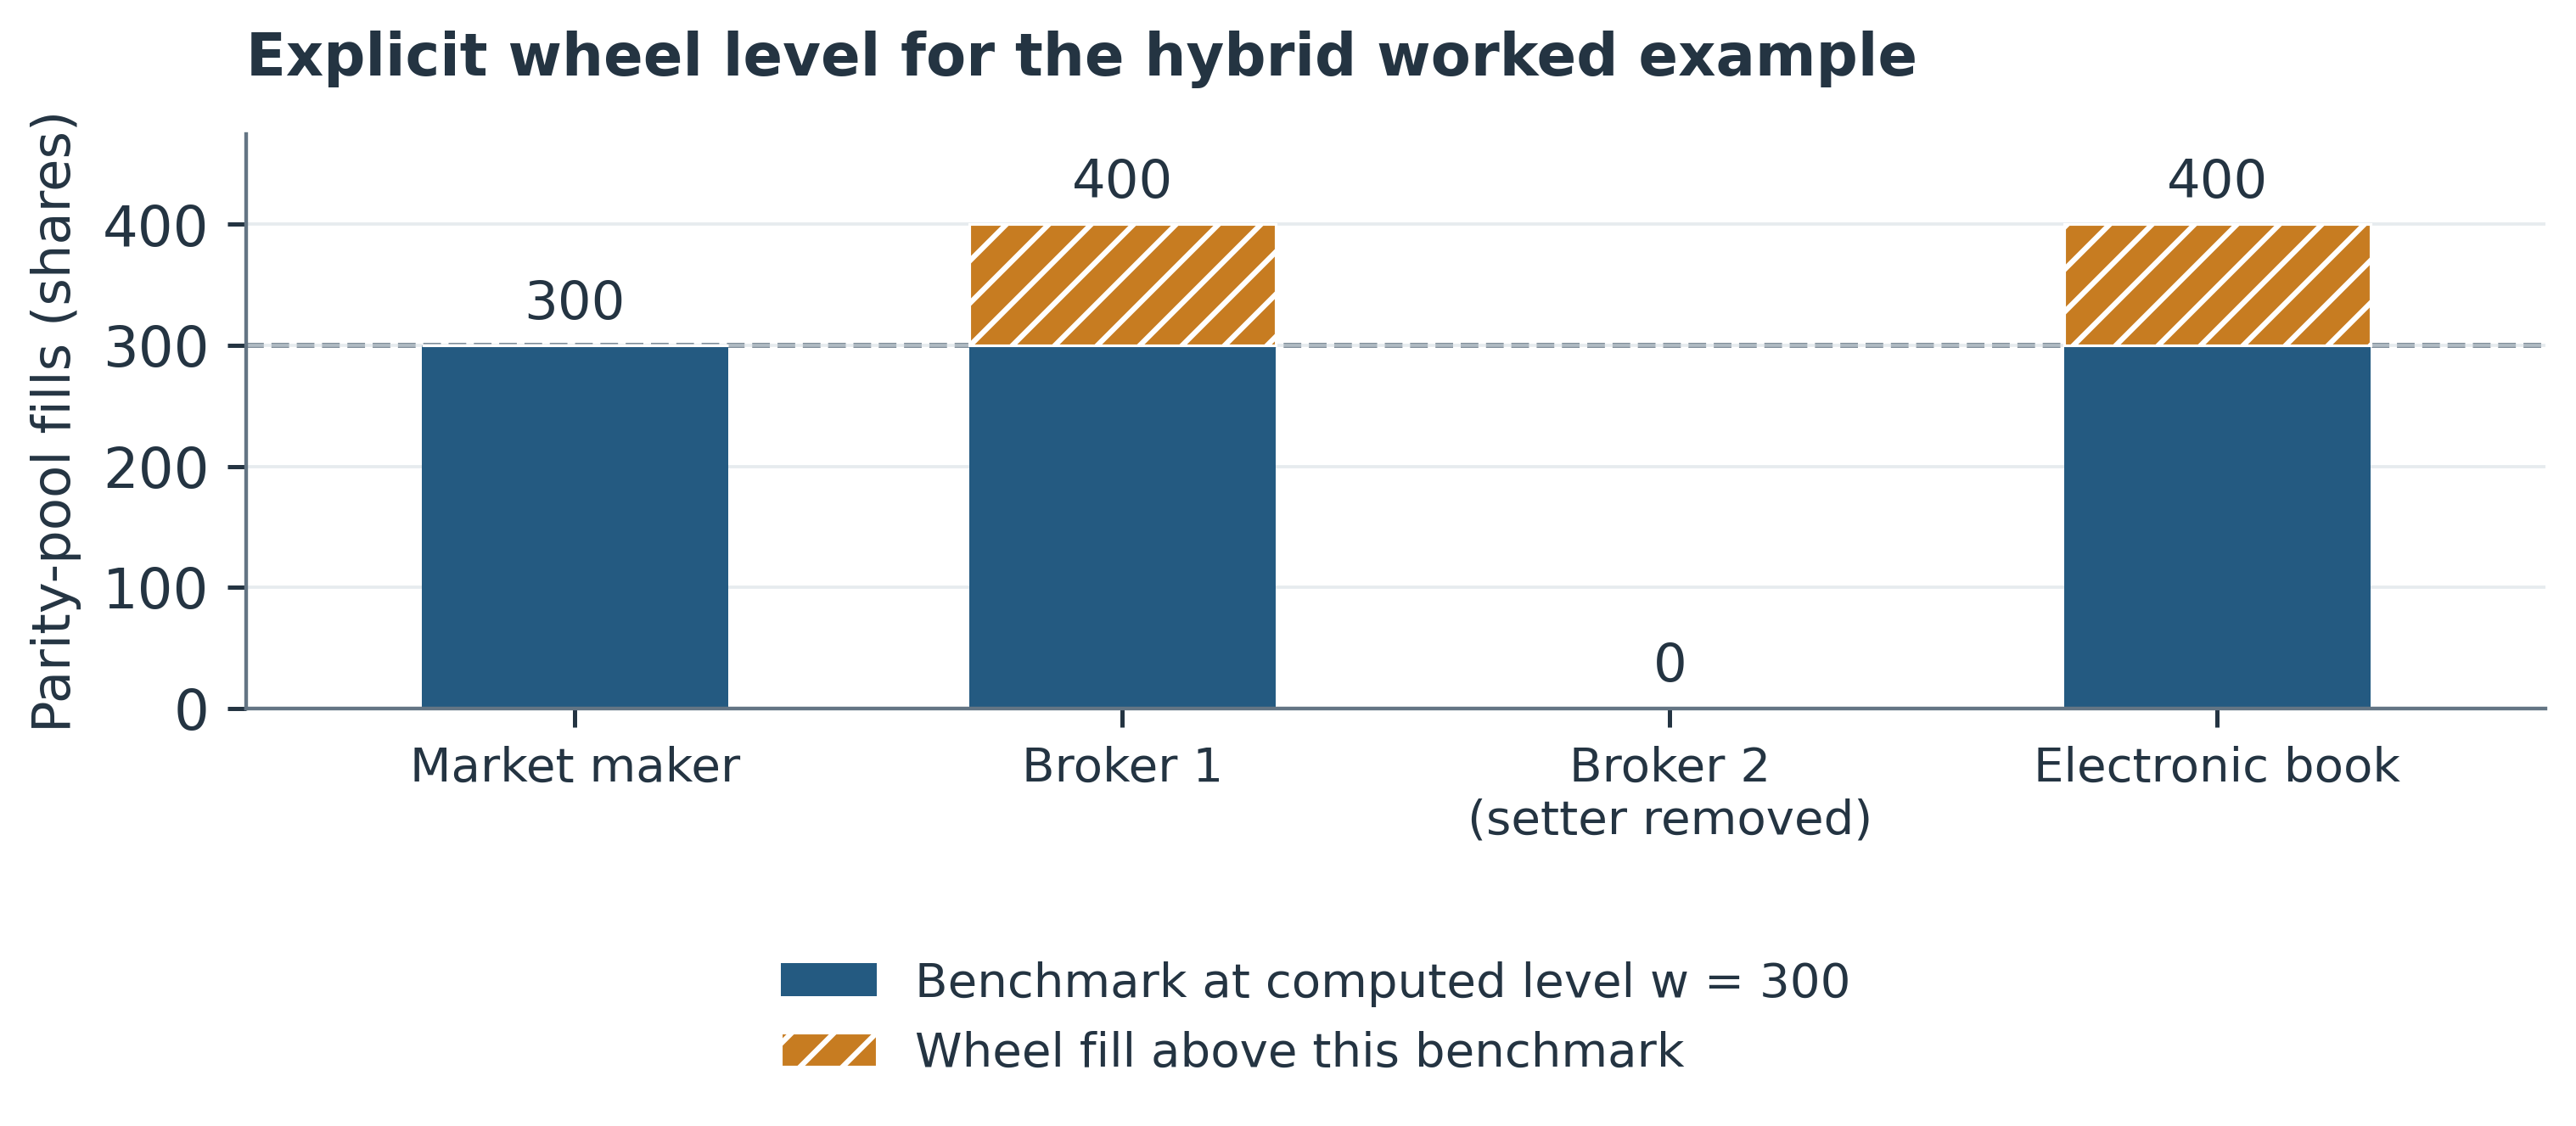
\includegraphics[width=\linewidth]{figures/wheel_water_level.png}
\caption{The post-setter parity pool has claims $(300,500,0,1000)$, lot $L=100$, and incoming quantity 1,100. With fuel 20, \lean{wheelLevel} returns $w=300$, producing benchmark $(300,300,0,300)$ and wheel fills $(300,400,0,400)$. The coordinate differences $(0,100,0,100)$ are at most one lot. The different benchmark level $s=400$ clears all 1,100 shares and coincides with the wheel in this example; the theorem uses the explicitly computed $w$.}
\label{fig:band}
\end{figure}

\FloatBarrier
\begin{corollary}[Vanishing-lot analytic limit]\label{thm:continuum}
Fix a participant count $m\ge1$. For run $k$, let $Q^{(k)}\in\N^m$, lot $L_k$, fill vector $a^{(k)}$, and executable water level $w_k$ be the quantities in Theorem~\ref{thm:within}. For any real scale $c_k>0$,
\[
 \max_{1\le i\le m}\left|
 \frac{a_i^{(k)}}{c_k}-
 \min\!\left\{\frac{Q_i^{(k)}}{c_k},\frac{w_k}{c_k}\right\}
 \right|\le \frac{L_k}{c_k}.
\]
Consequently, if $L_k/c_k\to0$, the normalized wheel allocations converge uniformly to their constrained-equal-awards profiles. If also $Q_i^{(k)}/c_k\to q_i$ for every $i$ and $w_k/c_k\to s$, then $a_i^{(k)}/c_k\to\min\{q_i,s\}$ for every participant.
\end{corollary}
\begin{proof}
The machine-checked finite inequality in Theorem~\ref{thm:within} gives
$|a_i^{(k)}-\min\{Q_i^{(k)},w_k\}|\le L_k$ for each $i$. Embed the natural numbers in $\mathbb R$, divide by $c_k$, and take the maximum over the fixed finite set of participants. The first limit follows by squeezing. The second follows from continuity of $\min$.
\end{proof}
This real-valued limit is an analytic corollary of the checked integer bound, not an additional Lean declaration. It identifies the precise asymptotic regime: the lot must vanish relative to the economic scale, not necessarily in absolute shares.

\begin{theorem}[Impossibility; \lean{serial\_band\_incompatible}, \lean{ex\_incompatible}]\label{thm:impossible}
Let two participants hold $q_1\ge x$ and $q_2>0$ with $L<x$. Every allocation satisfying Axioms~\ref{ax:feas} and~\ref{ax:serial} is $(x,0)$, which violates Axiom~\ref{ax:band} for every water level. Instance: sizes $(200,200)$, $L=100$, $x=200$.
\end{theorem}
Within these definitions, seriality and the band condition are jointly unsatisfiable on the stated family of two-order instances. A hybrid can apply serial priority to a setter tranche and a banded allocation to a separate residual pool; the theorem does not classify every priority feature of an actual venue.

\begin{theorem}[Ladder uniqueness; \lean{LadderSerial}, \lean{ptLadder}, \lean{ladder\_unique}]
Extend seriality across levels: a deeper level filled implies the shallower level filled in full. Any ladder allocation that is level-wise feasible and serial, and serial across levels, equals the price--time ladder.
\end{theorem}

\begin{remark}[Class versus point]
Axiom~\ref{ax:band} does not determine the allocation: the pointer is free, and distinct pointers can yield identical fills (Section~\ref{sec:obs}). The band therefore defines a compatibility class and a proved property of the modeled wheel, not a characterization of venue parity. By contrast, feasibility plus seriality characterize the modeled price--time output.
\end{remark}

\section{Structure theorems}\label{sec:structure}

\begin{theorem}[Conservation and caps; \lean{wheelRound\_sum}, \lean{wheelRound\_cap}, \lean{wheelRound\_le\_L}, \lean{wheel\_sum}, \lean{wheel\_cap}, \lean{rule737\_sum}, \lean{rule737full\_sum}, \lean{priceTime\_cap}, \lean{priceTime\_sum\_le}]
At every tier, fills respect sizes, a wheel visit gives at most one round lot, and fills plus leftover equal the incoming quantity.
\end{theorem}

\begin{theorem}[Displayed precedence; \lean{t3\_only\_after\_t2}]\label{thm:dbh}
For the specific three-tier operator \lean{rule737full}, non-displayed interest receives quantity only after the displayed tier leaves positive quantity. The result concerns this three-tier operator, not every venue's allocation rule.
\end{theorem}

\begin{theorem}[Completeness; \lean{tot}, \lean{passS\_tot\_lt}, \lean{wheelS\_complete}, \lean{wheelS\_exhausts}, \lean{wheel\_exhausts}]\label{thm:complete}
With $L\ge1$, an un-truncated pass over a level with positive total remaining strictly reduces that total. Hence if quantity is left over, either the level is exhausted or fewer than $\tot$ passes were available; with fuel $\tot+1$, positive leftover forces exhaustion, and the fills then equal the displayed sizes.
\end{theorem}
At this canonical fuel bound, positive leftover certifies exhaustion of the level. With a smaller fuel bound it can instead reflect computational truncation.

\begin{theorem}[Price priority on a ladder; \lean{matchAsks}, \lean{matchAsks\_conserve}, \lean{price\_priority}, \lean{no\_fill\_above\_limit}]
A buy with limit $\ell$ walks the ask ladder over levels priced $\le\ell$, price--time within each. Fills plus leftover equal $x$; a level above the limit receives nothing; and if any deeper level receives quantity, every order at the top marketable level is filled in full.
\end{theorem}

\begin{theorem}[Price priority over parity; \lean{matchNYSE}, \lean{matchNYSE\_conserve}, \lean{nyse\_price\_priority}]
On a ladder of hybrid levels (price, setter tranche, parity sizes), with $L\ge1$ and fuel $\sum\text{parity}+1$ at the top marketable level: if any deeper level receives quantity, the top level's setter tranche was filled in full and its parity fills sum to its displayed size.
\end{theorem}
Price priority is seriality one level up. A serial venue is price--time on the ladder, each level price--time on its queue; a hybrid venue is price--time on the ladder, each level setter-then-parity on its queue.

\begin{example}[\lean{ex\_book}, \lean{ex\_nyse}]
Serial ladder $\{10.00{:}(200,300),\ 10.01{:}(400),\ 10.03{:}(500)\}$: a $700$-share buy with limit $10.01$ fills $(200,300)$ then $200$; with limit $10.00$ it fills $500$ and leaves $200$. Hybrid ladder $\{10.00{:}\ \text{setter }200,\ (300,500,0,1000)\},\ \{10.01{:}(400)\}$: a $2200$-share buy exhausts the first level ($200+1800$) and takes $200$ at $10.01$; a $1500$-share buy stops inside the first level with wheel fills $(300,500,0,500)$.
\end{example}

\begin{proposition}[Integer wheels need not preserve depth-share domination; \lean{wheel\_book\_share\_counterexample}]
Let the book be first, with sizes $(1000,100)$, lot $L=100$, and incoming quantity $x=100$. Both the pass wheel and the persistent pointer wheel give $(100,0)$. The book receives all executions while supplying only $1000/1100$ of the depth, and $100\cdot1100>1000\cdot100$. Thus the benchmark's multiplicative share inequality does not transfer unchanged to either integer wheel.
\end{proposition}

\begin{lemma}[Book share under water-filling; \lean{book\_share\_le\_depth\_share\_mem}]
Under water-filling at level $s$, if a participant of size $Q_b$ is uncapped ($s\le Q_b$) and at least as large as every other ($q_i\le Q_b$), then $\min\{Q_b,s\}\cdot\sum_iq_i\le Q_b\cdot\sum_i\min\{q_i,s\}$: its fill relative to the others' is at most its depth relative to theirs.
\end{lemma}
Here the book is one of the participants, and its being largest and uncapped is an explicit hypothesis. The lemma concerns the water-filling benchmark; the preceding proposition isolates exactly why the finite-increment wheels differ.

\section{Allocation as rationing, and the pointer theorem}\label{sec:rationing}

\subsection{The identification}
A claims problem is a vector of claims $c\in\N^m$ and an amount $E\le\sum c$ to divide; a rule assigns awards $a\le c$ summing to $E$ \citep{young1987,young1994,thomson2003}. A queue at a price with incoming quantity $x$ is a claims problem with claims $q$ and amount $\min\{x,\sum q\}$. Under this identification:
\begin{itemize}
\item price--time is the \emph{sequential priority} rule for the arrival order \citep{moulin2000};
\item constrained equal awards (called water-filling in the executable kernel) assigns $\min\{q_i,s\}$ \citep{herrero2001};
\item the round-lot wheel is a finite-increment mechanism with a constrained-equal-awards approximation guarantee and a rotation order, related to indivisible claims allocation \citep{herrero2008}.
\end{itemize}
Theorem~\ref{thm:unique} is then a characterization of sequential priority by seriality, Theorem~\ref{thm:within} a finite-increment approximation theorem for constrained equal awards, and Theorem~\ref{thm:impossible} an incompatibility result for the stated priority and balance axioms. The rationing literature supplies a further composition requirement.

\begin{axiom}[Composition; \citealp{moulin2000}]\label{ax:comp}
Allocating $x$, then allocating $y$ against the residual claims, gives the same awards as allocating $x+y$ at once.
\end{axiom}
Composition is what makes an allocation rule well defined on a \emph{stream} of executions rather than on a single one. An exchange processes incoming orders one at a time; without composition, the fills a resting order receives would depend on how the contra-side quantity happened to be chopped into orders.

\begin{definition}[Stateful stream consistency]
For a transition system, the analogous property compares final states: running $x$ and then $y$ should agree with running $x+y$, subject to the termination conditions of the executable transition system. This is distinct from Axiom~\ref{ax:comp}, whose domain contains only residual claims.
\end{definition}

\subsection{What composes, and on which index}
\begin{theorem}[Estate composition and level composition]
\emph{Lean: \lean{priceTime\_comp}, \lean{waterFill\_level\_comp}, and \lean{waterFill\_two\_equal\_no\_single\_share}.}
Price--time satisfies estate composition (Axiom~\ref{ax:comp}):
\[
\lean{priceTime}\,Q\,(x+y)
=\lean{priceTime}\,Q\,x
\oplus\lean{priceTime}\,(Q\ominus\lean{priceTime}\,Q\,x)\,y.
\]
The benchmark instead satisfies a \emph{water-level} identity,
$\min\{q,s+t\}=\min\{q,s\}+\min\{q-\min\{q,s\},t\}$ pointwise. This identity is not Axiom~\ref{ax:comp} on an integer estate domain: for claims $(10,10)$, every natural water level clears an even number of shares, so no level represents the one-share estate. Thus natural water levels do not parameterize the full integer estate domain $0\le E\le\sum q_i$.
\end{theorem}

\begin{theorem}[Estate-indexed completion and the reset obstruction; \lean{discreteCEA\_feasible}, \lean{discreteCEA\_reset\_not\_composable}]\label{thm:discrete-cea}
Define $\lean{discreteCEA}\,Q\,E$ by running the unit-increment wheel on claims $Q$ and estate $E$, with a claims-determined fuel bound. For every $Q$ and $E$, this allocation is feasible: it respects every claim and awards exactly $\min\{E,\sum_iq_i\}$. It therefore completes the integer estate domain omitted by natural water levels. But if its deterministic rotation is reset for each estate, it fails Axiom~\ref{ax:comp}: on $Q=(10,10)$, one unit followed by one unit yields $(2,0)$, whereas the two-unit estate yields $(1,1)$.
\end{theorem}
A deterministic tie-break that restarts from a fixed participant is an exact indivisible allocation rule for each estate, yet not a stream-consistent rule on residual claims. Persisting its rotation produces the stateful wheel below and restores conditional stream consistency; it does not turn the stateful theorem into the stateless Axiom~\ref{ax:comp}.

\subsection{The pass-reset wheel does not}
\begin{theorem}[\lean{wheel\_not\_path\_independent}]
Two participants of $300$, $L=100$. Allocating $100$ and then $100$, restarting the pass at the pointer each time, gives $(200,0)$; allocating $200$ at once gives $(100,100)$.
\end{theorem}
The pass-reset wheel begins each execution with a fresh pass at the first participant. It is banded (Theorem~\ref{thm:band}) and conservative, but it is not path independent, and a resting order's fill under it depends on the chopping of the contra flow.

\subsection{The pointer-and-lot wheel does}
Let the state carry, in addition to each participant's (allocated, remaining), the rotation itself---the internal list is kept rotated so that its head is the pointer---and the round-lot allowance still owed to the head (\lean{WState}). A visit (\lean{stepW}) rotates the dead prefix to the back (\lean{findLive}), gives the live head $\min\{\mathrm{lot},\min\{r,x\}\}$, and either advances the pointer and resets the allowance to $L$ (when the visit completed the lot or exhausted the participant) or stays with the allowance reduced (when the incoming quantity ran out mid-lot). A run (\lean{runW}) iterates visits until quantity or remaining size is exhausted. Participant identifiers are preserved through rotation; output comparisons are made after restoring canonical label order.

\begin{theorem}[Balance of the pointer wheel; \lean{AllAtP}, \lean{AllAtP\_band}, \lean{stepW\_allAtP}, \lean{runW\_band}, \lean{runW\_balanced}]\label{thm:pointer-band}
For $L>0$, every state returned by a fuel-bounded \lean{runW} execution initialized with zero allocations satisfies the band predicate for some $w$: all allocations are at most $w+L$, and every unexhausted participant has allocation at least $w$. Exhausted participants may lie below $w$. Consequently, no participant is more than one round lot ahead of an unexhausted participant. This is the same \lean{runW} operator used in Theorem~\ref{thm:pointer}.
\end{theorem}
\begin{proof}[Proof idea]
The pointer-relative invariant \lean{AllAtP} records a low-then-high cycle boundary. The current live head has allocation plus unused lot allowance exactly $w+L$; participants not yet visited in the cycle remain at $w$, participants already visited are at $w+L$, and exhausted records never exceed that ceiling. A partial visit reduces the allowance by exactly the fill, a completed visit moves the head across the boundary, and completing a cycle raises $w$ by $L$. Thus every visit preserves the invariant, which implies the band.
\end{proof}

\begin{lemma}[Step composition; \lean{stepW\_split}]
Against a non-exhausted state, either the first visit with $x$ and with $x+y$ coincide, or the visit with $x$ is partial and the visit with $x+y$ equals the visit with $y$ from the partial state, with fills adding.
\end{lemma}

\begin{theorem}[Path independence of the pointer wheel; \lean{runW\_stable}, \lean{runW\_comp}]\label{thm:pointer}
Let $r_1=\lean{runW}\ L\ n_1\ st\ x$ and $r_2=\lean{runW}\ L\ n_2\ r_1.1\ y$. If $r_1.2=0$ and $\lean{Stopped}\ r_2.1\ r_2.2$, then
\[
\lean{runW}\ L\ (n_1+n_2)\ st\ (x+y)=r_2.
\]
Thus a first run that fully allocates $x$, followed by a terminating run of $y$, agrees exactly with the combined run at the summed fuel. The theorem is uniform in the round lot, participant count, pointer position, and partially consumed current lot; it does not remove its completion, termination, or fuel hypotheses.
\end{theorem}
\begin{proof}[Proof idea]
Induction on the fuel of the first run. Each visit is either identical in the split and joint runs (the lemma's first case), in which case the induction hypothesis applies to the residual, or partial (the second case), in which case the first run has ended with quantity zero, the joint run's next visit is exactly the second run's first visit, and the remaining visits agree by the stability of terminated runs under extra fuel.
\end{proof}

\begin{corollary}[Canonical stream consistency on reachable states; \lean{runWFull}, \lean{runWFull\_comp\_reachable}]\label{thm:pointer-full}
Let $st$ be any state returned by \lean{runW} from \lean{initW}, and let \lean{runWFull} choose fuel $\lean{totW}(st.S)+1$. If $L>0$ and the first estate satisfies $x\le\lean{totW}(st.S)$, then for every $y$,
\[
\lean{runWFull}\ L\ st\ (x+y)
=\lean{runWFull}\ L\ (\lean{runWFull}\ L\ st\ x).1\ y.
\]
The reachable-state allowance invariant makes positivity automatic. The supporting descent and conservation lemmas prove that canonical fuel terminates and that the first admissible estate clears. Allowance positivity, completion, and stopping therefore follow from reachability, canonical fuel, and the first-estate bound. The lower-level theorem \lean{runWFull\_comp} covers arbitrary supplied states and therefore retains a positive-current-allowance premise to exclude malformed states with allowance zero.
\end{corollary}

\begin{example}[\lean{pointer\_wheel\_instance}, \lean{pointer\_wheel\_odd\_instance}]
On the counterexample above, the persistent wheel allocates $100$ then $100$ as $(100,100)$, the same as $200$ at once; $150$ then $150$ gives the same state as $300$ at once, the partial lot carrying across the boundary.
\end{example}

Figure~\ref{fig:composition} compares reset and persistent executions and records a partial-lot transition.

\begin{figure}[tbp]
\centering
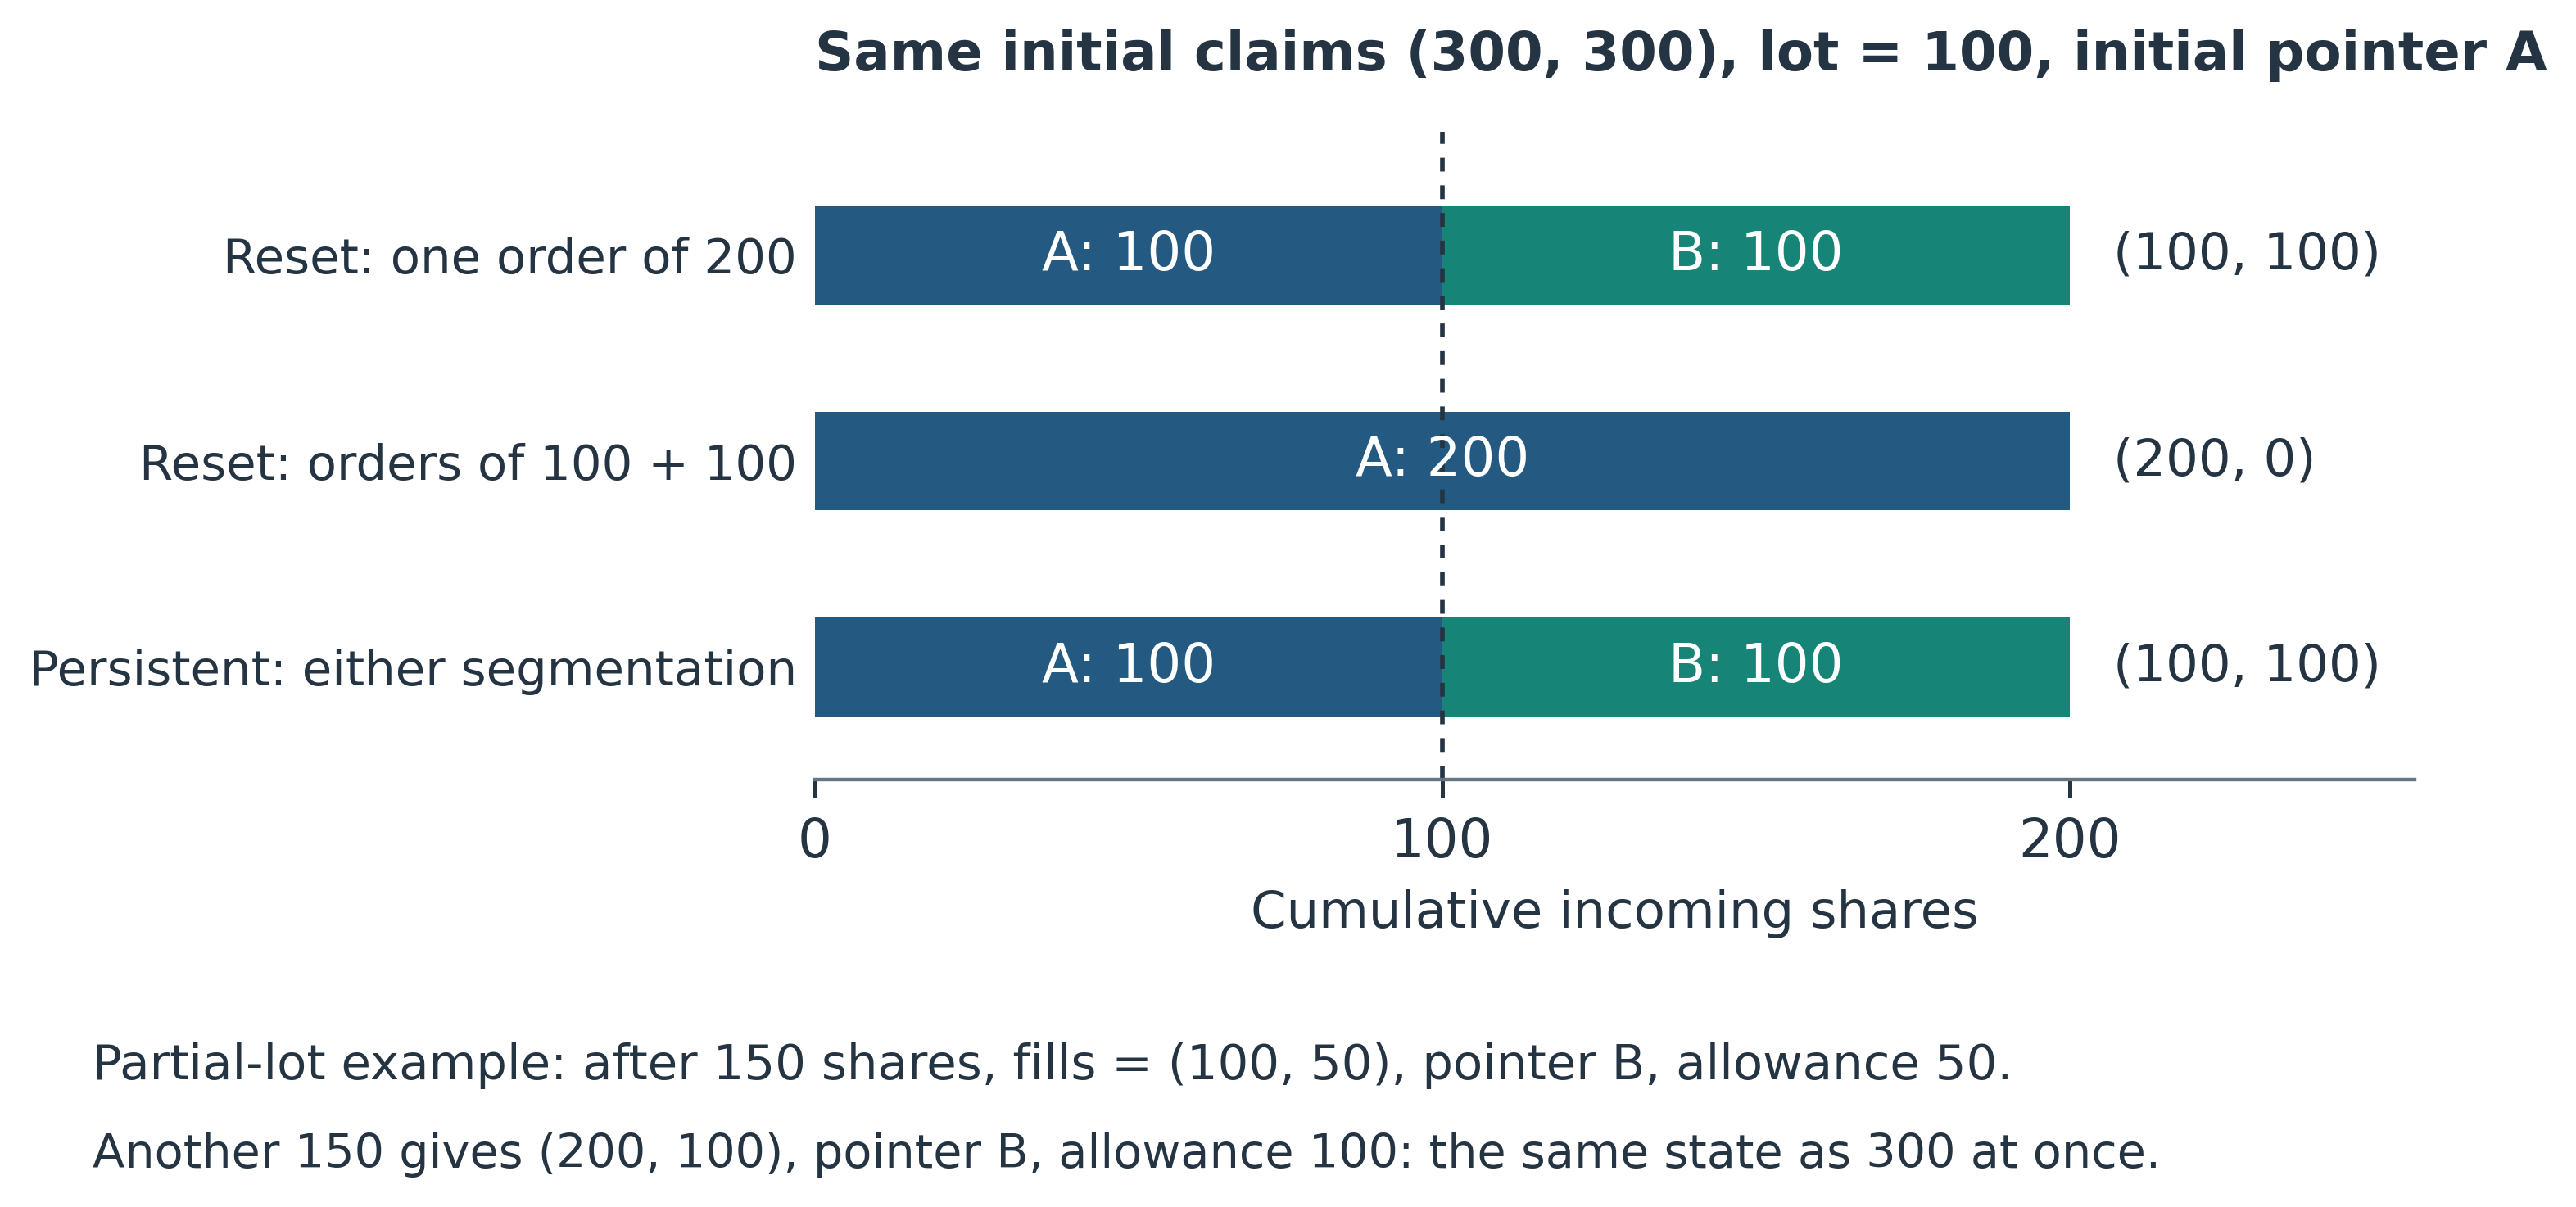
\includegraphics[width=\linewidth]{figures/stream_composition.png}
\caption{Segmentation changes a reset wheel but preserves the modeled persistent wheel. Start with claims $(300,300)$, lot 100, and pointer A. One 200-share estate gives $(100,100)$; two reset 100-share estates give $(200,0)$. The persistent wheel gives $(100,100)$ in both cases. The partial-lot example also preserves the complete state: 150 followed by 150 agrees with 300 at once. Fills and state labels are restored to the fixed external order $(\mathrm A,\mathrm B)$.}
\label{fig:composition}
\end{figure}

\subsection{What the theorem establishes}
Exchange documentation specifies that parity allocation proceeds from an allocation wheel and that the wheel advances across executions \citep[questions 7--8]{nyse2024parity}. The FAQ supports persistent rotation; it does not establish this paper's particular partial-lot carry rule or equivalence to the complete exchange engine. Theorems~\ref{thm:pointer-band} and~\ref{thm:pointer-full} place balance and exact split/combined equality on one executable construction. Example~\ref{thm:pointer-necessary}, Theorem~\ref{thm:fiber-pointer}, and Theorem~\ref{thm:saturated-quotient} below use explicit, different observation contracts: the four-party collision requires pointer information beyond queue and fills; the fiber theorem gives exact pointer necessity and sufficiency conditional on a common authenticated observation; and the $mL$ result bounds a complete predictive summary without separate side inputs. Corollary~\ref{cor:allowance-recovery} proves that cumulative allocation determines the allowance on every reachable live-head state. These statements concern the modeled wheel and do not characterize all banded stream-consistent mechanisms.

\plain{If a 200-share execution is processed as two consecutive 100-share executions, a stream-consistent mechanism should end in the same state either way. A wheel that forgets its position can fail. The persistent wheel passes this test for every reachable state and admissible first estate. Its unused allowance can always be recovered from the cumulative fill at the current pointer; the pointer label remains the phase datum that aligned fills do not necessarily reveal.}

\section{Cross-market structure}\label{sec:cross}

\subsection{Consolidation}
The definitions in this section are executable analytic kernels for selected Regulation NMS concepts. The integrated regulatory specification in Section~\ref{sec:clauses} supplies the definitions, exceptions, procedural duties, and versioned parameters needed for clause traceability. Unless stated otherwise, numerical parameters describe the operational compliance regime on September~5, 2026 \citep{sec2005regnms,sec2025relief,ecfr2026regnms}.
\begin{definition}[\lean{nbo}, \lean{nboSH}]
The model NBO is the minimum protected offer across the supplied venue-top quotations. A quote is protected only when it is automated, at the venue top, and at least the supplied round-lot size $L$.\footnote{The parameter $L$ is security-specific, not a universal 100-share constant. Rule~600(b)(93) assigns 100 shares when the prior evaluation-period average closing price is at most $250$, 40 shares from $250.01$ through $1{,}000$, 10 shares from $1{,}000.01$ through $10{,}000$, and one share above $10{,}000$; a new NMS stock receives 100 shares. The compliance date for this round-lot definition was November~3, 2025. The October~2025 relief concerned exchanges' conforming rule-change filings, not postponement of the tiered definition itself. The examples use $L=100$, while the theorems are uniform in $L$ \citep{ecfr2026regnms,sec2024nms,sec2025relief}.} Under the modeled self-help exception, the affected venue's quotations are excluded.
\end{definition}
\begin{theorem}[\lean{nbo\_le\_protected}, \lean{oddlot\_not\_protected}, \lean{selfhelp\_raises\_nbo}]
Every protected offer is at or above the NBO; an odd-lot or manual quote is never protected and never sets it; removing a venue's quotes can only raise it.
\end{theorem}
\begin{example}[\lean{ex\_nbo}]
With $L=100$, venue $v_1$ supplies an automated 300-share offer at $10.02$; $v_2$ an automated 50-share offer at $10.01$; $v_3$ a manual 200-share offer at $10.01$; and $v_4$ an automated 500-share offer at $10.03$. The model NBO is $10.02$.
\end{example}

\subsection{Order protection}
\begin{definition}[\lean{tradeThroughBuy}, \lean{sweepThenExecute}]
In the model, a buy executed above the NBO is a trade-through. The sweep operator sends an intermarket sweep to each supplied protected quotation better than execution price $px$, filling $\min\{\text{size},x\}$ in list order, then records the remainder at $px$.
\end{definition}
\begin{theorem}[\lean{compliant\_of\_le}, \lean{route\_to\_nbo\_no\_trade\_through}, \lean{sweep\_conserve}, \lean{iso\_compliance}]
Execution at or below the NBO is compliant. Sweep fills plus quantity executed at $px$ equal $x$, and if any quantity is executed at $px$ then every better protected quote received a sweep for exactly its size.
\end{theorem}
\begin{example}[\lean{ex\_sweep}]
On the quotes above, a $1000$-share sweep at $10.03$ sends $300$ to $v_1$ and executes $700$ locally.
\end{example}
The local remainder is not capped by modeled venue liquidity. The code also omits the one-second window, flickering-quotation treatment, quotation availability and timing, and Rule~611 exceptions other than the modeled ISO and self-help cases. Accordingly, \lean{iso\_compliance} is a theorem about this abstraction rather than certification of full Rule~611 compliance.

\subsection{Tick, lock, fee}
\begin{definition}[\lean{rule612}, \lean{notLockedOrCrossed}, \lean{slideBuy}, \lean{feeCap}, \lean{netCost}]
Under the legacy parameterization encoded here, quotes at or above $\$1$ are in whole cents and the access-fee cap is $\$0.003$ per share. The NBB is strictly below the NBO; a buy that would lock is displayed one modeled tick below the NBO; net cost is price plus fee.
\end{definition}
\begin{theorem}[\lean{effective\_tick}, \lean{relative\_tick\_antitone}, \lean{slide\_no\_lock}, \lean{slide\_le\_limit}, \lean{netCost\_le\_cap}, \lean{fee\_adjusted\_spread}]
Tick compliance plus no lock or cross forces a quoted spread of at least one cent at or above $\$1$; the relative tick is non-increasing in price; sliding never locks and never exceeds the limit; the fee-adjusted spread exceeds the quoted spread by at most two fee caps.
\end{theorem}
The SEC adopted a conditional $\$0.005$ minimum increment and a $\$0.001$ access-fee cap in 2024 \citep{sec2024nms}. Relief granted in 2025 was extended on June~11, 2026: compliance with amended Rules~610(c) and 612, and with Rule~600(b)(89)(i)(F), is postponed until the first business day of November~2027 \citep{sec2025relief,sec2026relief}. Thus the analytic kernels \lean{rule612} and \lean{feeCap} encode the regime operative on the paper's September~2026 date, while the clause layer separately encodes both legacy-relief and delayed amended functions in \lean{minimumTick612} and \lean{accessFeeCap610}. The compatibility theorems \lean{rule612\_iff\_minimumTick612\_legacy} and \lean{feeCap\_eq\_accessFeeCap610\_legacy\_dollar} prove that the legacy clause branches reduce to the analytic kernels. A separate June~2026 proposal to rescind Rule~611 and Rule~610(e) remained a proposal on the paper's stated date \citep{sec2026proposal}.

\subsection{Two market-data clocks}
\begin{theorem}[\lean{sip\_ge\_venue}, \lean{sip\_order\_preserved}, \lean{sip\_order\_inversion\_exists}, \lean{sip\_inversion\_bound}]
Consolidated time is never earlier than venue time; equal latencies preserve order; inversions exist; an inversion requires the latency difference to exceed the venue-time gap.
\end{theorem}

\subsection{Order types}
\begin{theorem}[Selected order-type properties]
\emph{Lean: \lean{midpoint\_inside}, \lean{midpoint2\_strict\_inside}, \lean{mpl\_no\_trade\_through}, \lean{fillReserve\_conserve}, \lean{fillReserve\_replenish}, \lean{dOrder\_within}, \lean{dOrder\_compliant}, \lean{marketPeg\_no\_lock}, \lean{primaryPeg\_mono}, \lean{postOnly\_rests\_iff}, and \lean{postOnly\_never\_takes}.}
The grid-valued midpoint $\lfloor(\NBB+\NBO)/2\rfloor$ lies in $[\NBB,\NBO)$ when $\NBB<\NBO$; it need not be strictly above the NBB for a one-grid-unit spread. In doubled-price units, the exact midpoint $\NBB+\NBO$ is strictly inside every non-locked spread. The floored kernel never trades through. A reserve order's display plus reserve falls by exactly the fill, and replenishment occurs only when the display was exhausted, to at most the original display. A discretionary order executes within $[\text{display},\text{limit}]$ and is protection-compliant when its limit is at or below the NBO. A market peg with $0<\mathrm{offset}\le\NBO$ never locks; a primary peg re-prices monotonically with the NBB. A post-only order rests only strictly below the best contra quote and never removes liquidity.
\end{theorem}
These are one-step semantic kernels. In particular, \lean{fillReserve} performs at most one refresh. Repeated matching, queue re-entry, repricing, rejection, routing, and attribute compatibility are represented as explicit certification duties in \lean{ClauseComplete.lean}; they are not implied by the one-step arithmetic theorem. Nasdaq's priority rules distinguish displayed and non-displayed interest beyond the within-queue price--time primitive modeled here \citep{nasdaq2026equity4}.

\subsection{Bands and tests}
\begin{theorem}[\lean{luldBands}, \lean{lower\_le\_ref}, \lean{ref\_le\_upper}, \lean{bands\_widen}, \lean{limitState\_boundary}, \lean{shortSaleOK}, \lean{no\_short\_at\_or\_below\_nbb}, \lean{effSpread2}, \lean{eff\_le\_quoted}, \lean{effSpread2\_neg\_iff}, \lean{midpoint\_zero\_eff}]
Price bands $\mathrm{ref}\pm\lfloor\mathrm{ref}\cdot\mathrm{pct}/100\rfloor$ contain the reference and widen in the percentage; a limit state has one side of the market on a band. With the short-sale circuit breaker in effect a short sale executes only strictly above the NBB. The signed buy-side kernel $\lean{effSpread2}\,px\,nbb\,nbo=2px-(nbb+nbo)$ is evaluated in $\Z$: it is at most the quoted spread when $px\le nbo$, vanishes at an exact grid midpoint, and is negative exactly below the midpoint. It preserves below-midpoint magnitude; a complete Rule~605 statistic still requires side, order-class, time, and aggregation inputs.
\end{theorem}
The clause layer represents the LULD obligations in a record for reference recomputation, tiering, late-day changes, rounding, limit and straddle states, pauses, reopening, dissemination, policies, and operative overnight protection. It derives the Rule~201 ten-percent trigger, enumerates every short-exempt reason and its internal conditions, and represents the complete amended Rule~605 order-class and disclosure-column schema. The kernel \lean{effSpread2} alone is not a report generator; \lean{rule605Complies} checks whether a supplied report record contains every required component.

\section{Auction structure}\label{sec:auction}

\begin{definition}[\lean{demandAt}, \lean{supplyAt}, \lean{matchedAt}, \lean{imbalanceAt}, \lean{crossKey3}, \lean{crossPrice3}, \lean{dmmFacilitate}]
Orders are (limit, size). Demand at $p$ is the size of bids with limit $\ge p$; supply at $p$ the size of asks with limit $\le p$; matched volume is their minimum; imbalance is the pair of one-sided excesses. The clearing key encodes, lexicographically, matched volume, then $B-\mathrm{imbalance}$, then $D-|p-\mathrm{ref}|$, for bounds $B,D$; the auction price maximizes the key over candidates. The designated market maker absorbs residual imbalance up to a committed size.
\end{definition}
This is the proved generic lexicographic auction kernel. Clause-level NYSE and Nasdaq records separately require the full definitions, eligible-interest treatment, entry and cancellation windows, imbalance messages and schedules, collars, priority, uniform price, official-price publication, LULD and halt variants, DMM and floor responsibilities, and contingency procedures. Facilitation remains a two-number theorem; satisfaction of the wider procedural record requires external evidence.
\begin{theorem}[\lean{demandAt\_antitone}, \lean{supplyAt\_mono}, \lean{crossPrice\_maximizes}, \lean{crossPrice\_global}, \lean{crossPrice2\_lex}, \lean{crossPrice3\_lex}, \lean{dmm\_clears}, \lean{dmm\_conserve}]
Demand is antitone and supply monotone in price. Over a nonempty finite candidate list the clearing price maximizes matched volume; over the ask prices it is a global maximizer; with the two- and three-level keys, assuming $B$ bounds every candidate imbalance and $D$ bounds every candidate reference distance, it also minimizes imbalance and then reference distance among maximizers. Facilitation clears the residual when the commitment covers it and conserves quantity.
\end{theorem}
\begin{example}[\lean{ex\_cross}, \lean{ex\_auction}]
Bids $\{(10.02,500),(10.01,300),(10.00,400),(9.99,200)\}$, asks $\{(9.98,300),(10.00,300),(10.01,400),(10.03,500)\}$: the auction clears at $10.01$ with $800$ matched and a $200$-share sell imbalance ($10.00$ would match $600$, $10.02$ only $500$); with reference $10.00$ the three-criterion price is still $10.01$; a $200$-share residual against a $500$-share commitment clears.
\end{example}

Figure~\ref{fig:auction} displays the demand, supply, and matched-volume calculations in the example.

\begin{figure}[tbp]
\centering
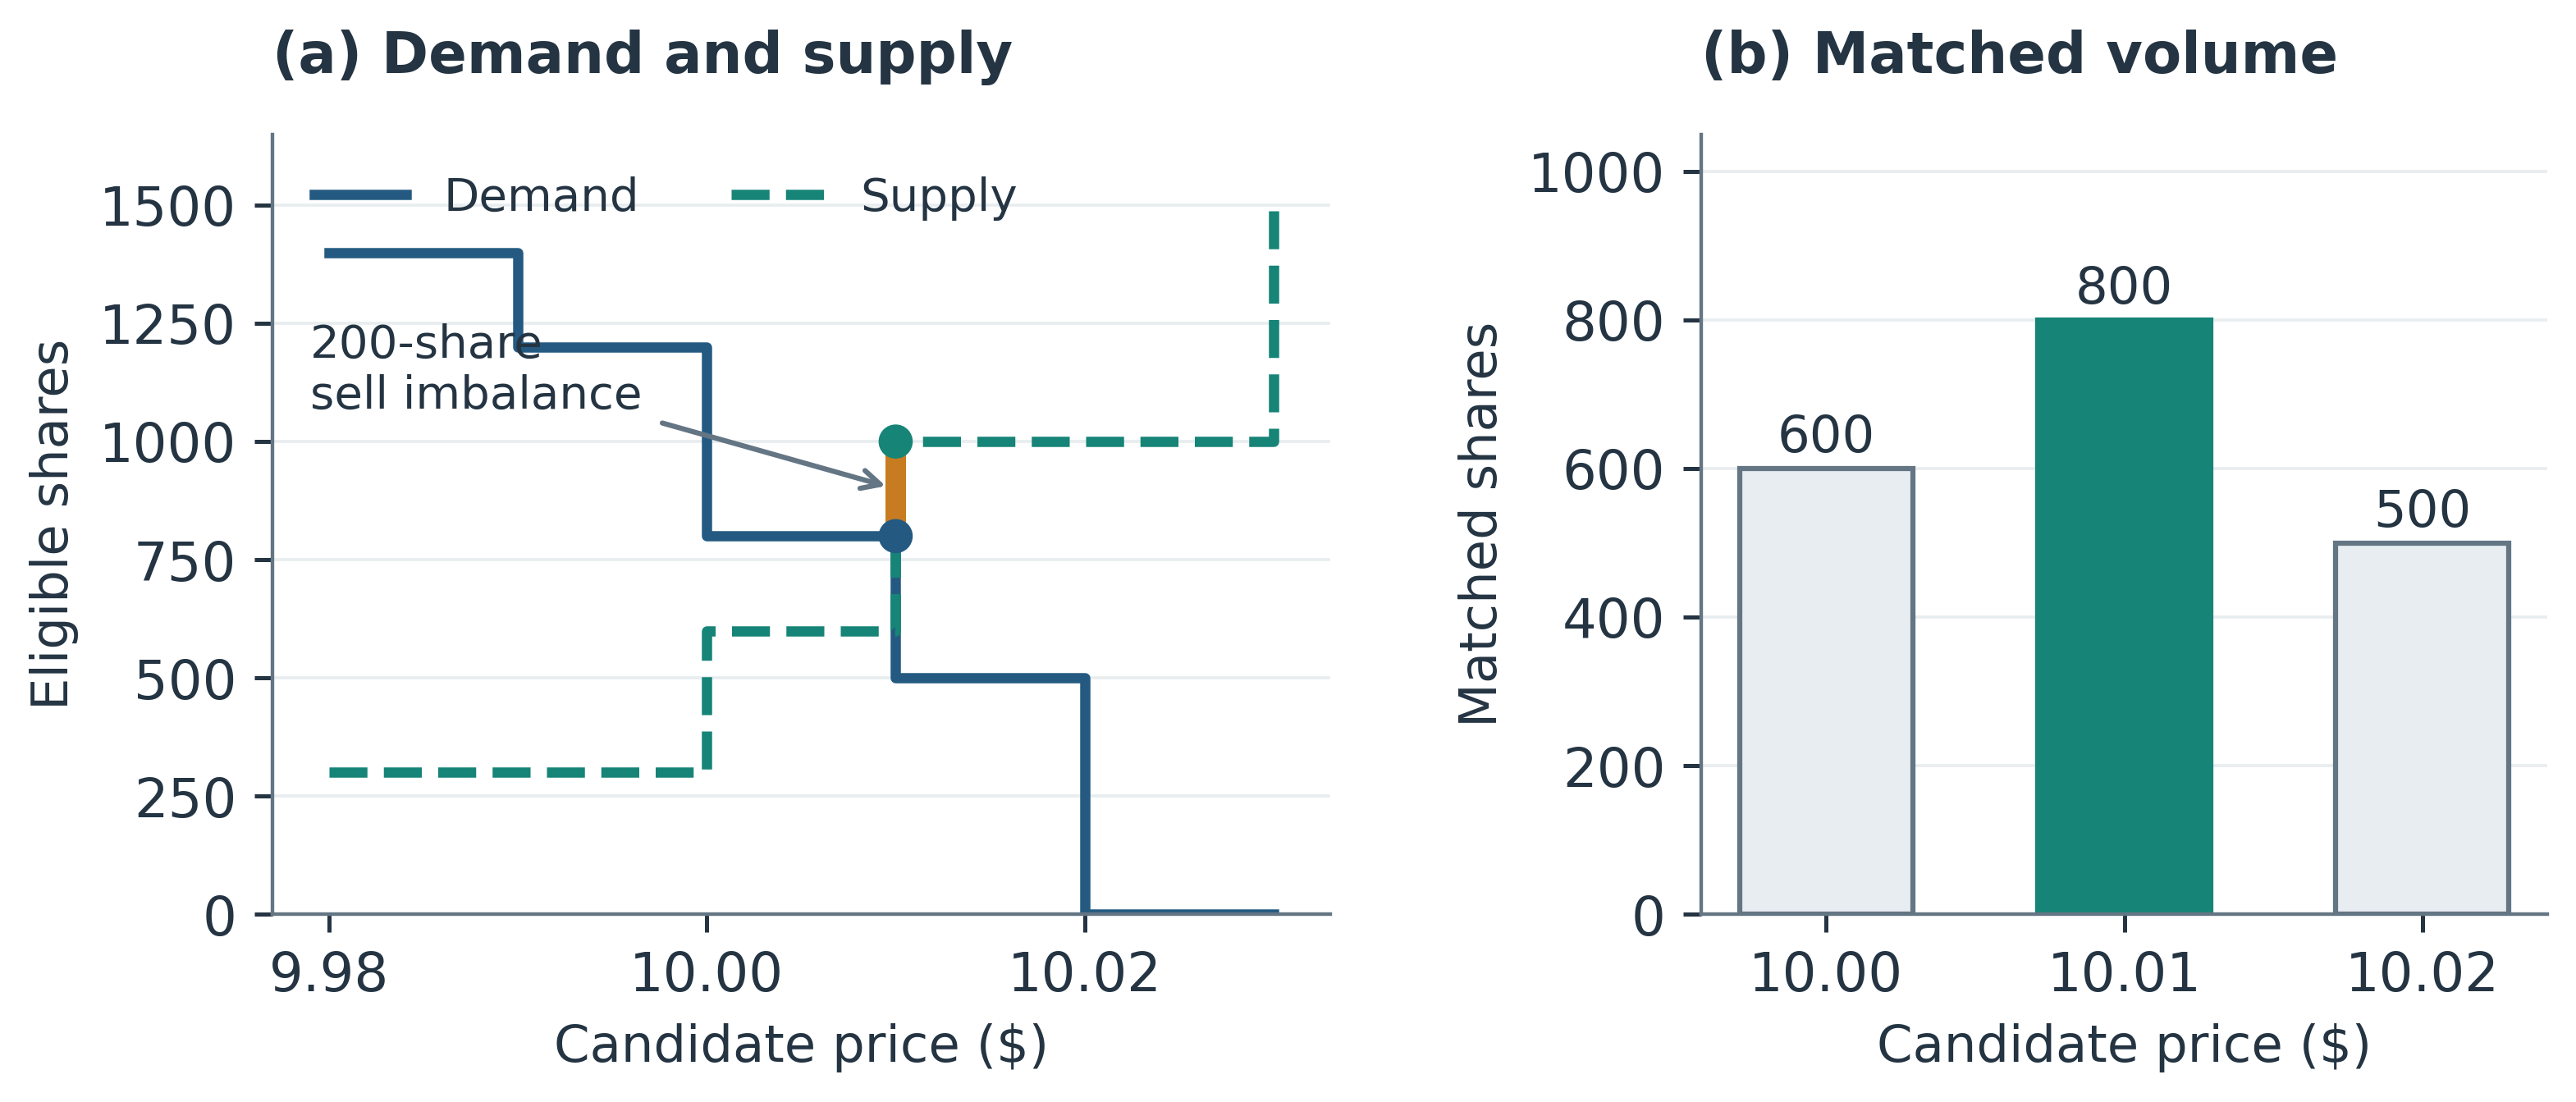
\includegraphics[width=\linewidth]{figures/auction_price_selection.png}
\caption{The auction example selects $\$10.01$: demand is 800 shares and supply 1,000, giving 800 matched and a 200-share sell imbalance. At $\$10.00$ and $\$10.02$, matched volumes are only 600 and 500. The step curves use the inclusive limit-price conditions in \lean{demandAt} and \lean{supplyAt}; the right panel compares three candidate prices.}
\label{fig:auction}
\end{figure}

\plain{An auction tests candidate prices. At each price it computes how many shares buyers and sellers could trade, selects the price with the greatest matched volume, then uses imbalance and distance from a reference price as tie-breakers. ``Lexicographic'' means applying those criteria in that fixed order, like sorting first by surname and then by given name.}

\newcommand{\StrategicAppendix}{%
\section{Certified inequalities for the strategic layer}\label{sec:strategic}

The following payoff comparisons use the stated allocation rules and additional behavioral assumptions. They are expressed with denominators cleared over $\Z$.

\subsection{Contests for a slot or a tranche}
$m$ contestants with linear effort cost compete for a prize $V$; effort $e'$ against others' total $O$ earns $\pi(e')=Ve'/(e'+O)-e'$ \citep{tullock1980}. Write $D=e+O$, $t=e'+O$.
\begin{theorem}[Best response; \lean{tullock\_best\_response}]\label{thm:tullock}
If $D=e+O$, $VO=D^2$, $t=e'+O>0$ and $D>0$, then $(Ve'-e't)D\le(Ve-eD)t$, i.e.\ $\pi(e')\le\pi(e)$ for every $e'\ge0$.
\end{theorem}
\begin{proof}[Proof idea]
$Dt\,[\pi(e)-\pi(e')]=D(D-t)^2$ under $VO=D^2$: a positive number times a square.
\end{proof}
\begin{theorem}[Symmetric equilibrium and dissipation; \lean{tullock\_symmetric\_foc}, \lean{tullock\_dissipation}, \lean{dissipation\_increasing}]
For $m\ge2$ and $V>0$, if a nonnegative integer $e$ satisfies $m^2e=(m-1)V$, then $e>0$ and the first-order condition holds at $O=(m-1)e$, total effort satisfies $m\cdot me=(m-1)V$, and $(m-1)(m+1)<m^2$: a fraction $(m-1)/m$ of the prize is dissipated and is strictly increasing in $m$.
\end{theorem}
\begin{example}[\lean{ex\_tullock}, \lean{ex\_tullock\_dev}]
$m=4$, $V=1200$: $e=225$, $D=900$, $O=675$, $VO=810{,}000=D^2$; the deviation $e'=300$ is unprofitable.
\end{example}

\subsection{The race for setter priority}
Two racers invest speed $b_1,b_2\ge0$ (sunk) for a tranche $S$; the faster wins, ties split. Doubled payoffs keep the model in $\Z$ (\lean{u2}).
\begin{theorem}[\lean{setter\_race\_no\_pure\_NE}, \lean{race\_spend}]
For $S\ge3$ no profile is a pure equilibrium: ties invite a one-unit raise, gaps of two or more invite undercutting, and a gap of one invites the loser to drop out or leapfrog. In every profile the doubled payoffs sum to $2S-2(b_1+b_2)$.
\end{theorem}
\begin{theorem}[Uniform mixture is an $\varepsilon$-equilibrium; \lean{sumU}, \lean{sumU\_closed}, \lean{uniform\_payoff}, \lean{uniform\_eps}, \lean{uniform\_selfpayoff\_zero}, \lean{uniform\_eps\_relative}]
For $N\ge1$, on the grid $\{0,\dots,N\}$ with prize $N$ and a uniform opponent, the $(N+1)$-scaled doubled payoff of bid $b$ is $N-2b$; the uniform strategy's own scaled payoff is $0$; the best pure deviation improves expected payoff by less than half a cost unit, and relative to the prize the gain is less than $1/N$.
\end{theorem}
These identities give the finite-grid dissipation result for the all-pay auction \citep{baye1996allpay}.

\subsection{Privileged slot and venue competition}
\begin{theorem}[Privileged-slot comparative statics]
\emph{Lean: \lean{dmm\_share\_antitone}, \lean{dmm\_option\_dilution}, \lean{dmm\_option\_spread}, and \lean{dmm\_advantage}.}
A free parity slot worth $\lfloor u/m\rfloor$ units times the half-spread $h$ is non-increasing in $m$ and non-decreasing in $h$; relative to a participant paying $c$ per slot, the advantage is exactly $c$.
\end{theorem}
\begin{theorem}[Routing; \lean{bestVenue\_le}, \lean{flowShare}, \lean{undercut\_wins}, \lean{fee\_cut\_captures}, \lean{fee\_gap\_bounded}]
The router's chosen net cost is at most every venue's; the venue with strictly lower net cost takes all marketable flow; a fee cut below the rival's net cost captures it; under the fee cap the net-cost gap at equal quoted prices is at most the cap.
\end{theorem}

\begin{principle}[Layering]
The strategic layer introduces additional behavioral assumptions. Its propositions are proved against the stated operators, while every translation from institutional rules to those operators remains a separately documented modelling assumption.
\end{principle}

}

\section{Observability structure}\label{sec:obs}

\begin{theorem}[Identification]
\emph{Lean: \lean{parity\_count\_fingerprint}, \lean{hidden\_depth\_lower\_bound}, and \lean{reserve\_certificate}.}
For an observer who knows $L$ and can delimit one un-truncated parity pass in a participant-aligned allocation record, if every participant holds at least a round lot then the pass fills are $(L,\dots,L)$ of length $m$: its length identifies the participant count. A public trade tape ordinarily lacks that participant alignment; without authenticated alignment, the known lot size, and the pass boundary, the theorem makes no surveillance claim. Separately, an execution of $x$ that clears a level certifies non-displayed depth of at least $x-Q^{\mathrm s}-\sum r_i$.
\end{theorem}

\begin{theorem}[Invisibility]\label{thm:invis}
{\raggedright\emph{Lean: \lean{priceTime\_zero}, \lean{priceTime\_tail\_invisible}, and \lean{priceTime\_boundary\_invisible}.}\par}
If $x\le q_1$, the queue-aligned price--time allocation vector is the same for every queue tail of the same length. More strongly, any two head sizes at least $x$, followed by equally long tails, generate the same vector. Thus aligned fills identify sizes only for a fully exhausted prefix; they give a lower bound for a partially filled marginal order and do not identify the remaining tail.
\end{theorem}
\begin{theorem}[No parity conformance from queue and aligned fills alone]\label{thm:no-parity-check}
{\raggedright\emph{Lean: \lean{parity\_pointer\_not\_identified\_from\_prints} and \lean{no\_parity\_conformance\_from\_queue\_and\_prints}.}\par}
For the participant-labelled queue $(300,500,200,1000)$, two distinct pointer states produce the same 1,100-share queue-aligned fill vector $(300,300,200,300)$ but reach distinct terminal states; the next 100-share allocation goes to different participants. Moreover, one identical candidate vector for the same queue conforms under one pointer and fails under the other. Therefore no Boolean function of the queue and aligned fills alone can be correct on both states: a parity conformance check must receive the pointer state or equivalent authenticated evidence.
\end{theorem}
\begin{example}[Four-party future-separation witness; \lean{FutureSufficient4}, \lean{future\_sufficient\_summary\_requires\_pointer\_information}]\label{thm:pointer-necessary}
Let $S$ map wheel states to an arbitrary summary type. Suppose there is a predictor that, for every four-party state and next quantity, correctly returns the next queue-aligned fill vector from only the current canonical queue, current aligned cumulative fills, $S(st)$, and that quantity. Then $S$ must assign different values to \lean{pointerA} and \lean{pointerC}. In particular, no universally future-sufficient summary can collapse the pointer distinction erased by queue and fills.
\end{example}
\begin{proof}[Proof idea]
The two witness states have the same canonical queue and zero cumulative fills. If their summaries were also equal, the predictor would receive identical inputs for the next 100 shares and would have to return the same vector. Evaluation proves that the actual next vectors differ, a contradiction.
\end{proof}

\begin{theorem}[General nondegenerate phase separation; \lean{ValidWheelPhase}, \lean{validWheelPhase\_probe\_equiv\_implies}]\label{thm:general-phase}
Let $st$ and $su$ each have a live head, a distinct live successor, a current allowance in $\{1,\ldots,L\}$, and more than $L$ shares remaining at every participant. Write their head pointer--allowance pairs as $(p,a)$ and $(q,b)$. If their participant-labelled new-fill vectors agree for every estate $x\le L$, then $p=q$ and $a=b$.
\end{theorem}
\begin{proof}[Proof idea]
The one-share probe identifies the head pointer. Once the pointers agree, suppose without loss that $a<b$. At estate $a+1$, the first state completes its allowance and gives the next share to its distinct successor, so $p$ receives $a$; the second state gives all $a+1$ shares to $p$. This contradicts probe equivalence. The hypotheses keep both probes away from exhaustion boundaries. The result is a necessity statement across arbitrary accumulated allocations, successor labels, and tails in this nondegenerate domain; equality of pointer and allowance alone does not erase differences in those other state components.
\end{proof}

Fix an arbitrary authenticated observation $O$ and an indexed family
$\{st_p:0\le p<m\}$. A summary $S$ is \emph{future sufficient on this
fiber} if one decoder, given $O(st_p)$, $S(st_p)$, a future estate $x$, and a
participant label $i$, returns the actual canonical next fill
$F_L(st_p,x)_i$ for every $p,x,i$ (\lean{WheelFiberSufficient}).

\begin{theorem}[Fiberwise pointer minimality; \lean{wheelFiberSufficient\_pointer\_injective}, \lean{wheelPointerCode\_fiber\_sufficient}]\label{thm:fiber-pointer}
Let $L>0$. Suppose every $st_p$ is a nondegenerate wheel phase whose live
head label is $p$, and $O(st_p)$ is the same for all $p<m$. Then every
future-sufficient summary $S$ is injective on the family:
\[
 S(st_p)=S(st_q)\quad\Longrightarrow\quad p=q.
\]
Conversely, the head label $p$ itself is a future-sufficient summary for the
fixed indexed family. Thus the pointer is an exact minimal predictive code on
this common-observation fiber: if all $m$ indices occur, precisely $m$ summary
values suffice and fewer cannot.
\end{theorem}
\begin{proof}[Proof idea]
If two summary values were equal, their observation inputs would also be
equal, so the common decoder would make the two states agree on every future
probe. Theorem~\ref{thm:general-phase} then forces their head labels to agree.
For sufficiency, the decoder uses the supplied head label to select the fixed
family member and executes \lean{nextWFill}. The necessity argument permits
arbitrary claims, accumulated fills, successors, tails, observation types,
summary types, and decoders satisfying the stated contracts; the converse is
relative to the fixed one-state-per-pointer family.
\end{proof}

\paragraph{A finite family of executable phase states.}
Fix $m\ge2$ and $L>0$. Label the participants $0,\ldots,m-1$ in cyclic order and give each original claim $2L+1$. For $0\le p<m$ and $1\le a\le L$, define $P_{p,a}=\lean{phaseState}\,m\,L\,p\,a$ by putting $p$ at the head, with record $(p,L-a,L+1+a)$ and current allowance $a$. Every other label follows in cyclic order with record $(i,0,2L+1)$. The declarations \lean{phaseState\_length}, \lean{phaseState\_labels\_unique}, \lean{phaseState\_capacities}, and \lean{phaseState\_claims\_large} verify the participant count, distinct labels, common original capacities, and remaining claims strictly above $L$. Moreover, \lean{phaseState\_reachable} proves that $P_{p,a}$ is reached by initializing that cyclic queue at $p$ and running $L-a$ shares with \lean{runWFull}.

Write $F_L(st,x)_i$ for the new allocation to label $i$ produced by \lean{runWFull}; the executable definition \lean{nextWFill} subtracts that label's cumulative allocation before the run from its allocation afterward. Define $st\sim_L su$ when $F_L(st,x)_i=F_L(su,x)_i$ for every $x$ and label $i$ (\lean{WheelFutureEquivalent}). A complete predictive summary has a decoder for those fills from the summary and $(x,i)$ alone, with $m,L$ fixed; it receives no separate queue or cumulative-fill input (\lean{WheelPhaseSufficient}).

\begin{theorem}[Finite executable phase identification and minimal predictive summaries]\label{thm:saturated-quotient}
{\raggedright\emph{Lean: \lean{phaseState\_probe\_equiv\_iff}, \lean{phaseState\_future\_equiv\_iff}, \lean{wheelPhaseSufficient\_injective}, and \lean{wheelPhaseCode\_sufficient}.}\par}
For the valid phases above,
\[
 P_{p,a}\sim_L P_{q,b}\quad\Longleftrightarrow\quad(p,a)=(q,b).
\]
It is enough to compare estates $x\le L$. Every complete predictive summary is injective on these $mL$ reachable states, and the code $(p,a)$ is sufficient. Hence the family has exactly $mL$ behavioral classes and any fixed-length binary encoding of a complete predictive summary needs at least $\lceil\log_2(mL)\rceil$ bits.
\end{theorem}
\begin{proof}
The actual canonical wheel gives its first share to $p$ (\lean{phaseState\_first\_fill}), so different pointers are separated by $x=1$. For equal pointers and $a<b$, take $x=a+1\le L$. In $P_{p,a}$, the first $a$ shares finish the current allowance and the successor receives one share; $p$ receives $a$ (\lean{phaseState\_allowance\_probe}). In $P_{p,b}$, all $a+1$ shares go to $p$ (\lean{nextWFill\_head}). These conclusions use \lean{runWFull} and its composition theorem directly. The case $b<a$ is symmetric. Equal phases reconstruct equal finite states, so all subsequent executions agree. A decoder cannot give the same code to two states separated by a probe; conversely \lean{wheelPhaseCode} records the head label and allowance and reconstructs the family member. Lean checks reachability, the separating executions, equivalence, injectivity, and sufficiency. Counting the $m$ pointer values and $L$ allowance values gives the cardinality; $2^b\ge mL$ gives the stated binary-encoding corollary.
\end{proof}

This uses the future-distinguishability principle underlying automaton minimization \citep{nerode1958}, applied to a specified reachable family of finite \lean{WState} values. Equivalence on every finite quantity stream gives the same classes: a single-estate stream supplies each separating probe, while equal phases give identical initial states and therefore identical streams. It does not characterize every banded mechanism or minimize all raw \lean{WState} representations. One-live-participant states, exhausted claims, and dead-prefix representations can erase distinctions elsewhere.

\begin{corollary}[Reachable allowance-phase identity; \lean{runW\_allowance\_phase}, \lean{allowance\_from\_cumulative}]\label{cor:allowance-recovery}
Fix $L>0$ and any execution of \lean{runW} from \lean{initW}. If the returned state has a live head $p$ with cumulative allocation $A_p$, then its current allowance is
\[
 a=L-(A_p\bmod L).
\]
Thus knowing the pointer and its aligned cumulative allocation determines the allowance on every reachable live-head state; no cycle-phase premise is supplied by the caller. The supporting invariant \lean{runW\_atWheelPhase} proves $A_p+a=kL+L$ for some $k$, and \lean{allowance\_from\_cumulative} discharges the arithmetic identity.
\end{corollary}

\begin{corollary}[Exact pointer state with aligned cumulative fills; \lean{phaseState\_full\_observation}, \lean{phaseState\_full\_summary\_injective}, \lean{phaseState\_full\_pointer\_sufficient}]\label{cor:pointer-exact}
For $m\ge2$ and $L>0$, restrict to the reachable full-allowance states
$\{P_{p,L}:0\le p<m\}$. Their original capacities are all $2L+1$, and their
participant-aligned cumulative-allocation observation is the identical vector
$(0,\ldots,0)$. Every future-sufficient extra summary must distinguish all
$m$ pointers, and the pointer label itself is sufficient. The exact extra-state
count on this authenticated-observation fiber is therefore $m$; any
fixed-length binary encoding needs at least $\lceil\log_2 m\rceil$ bits.
\end{corollary}

The identity in Corollary~\ref{cor:allowance-recovery} explains why the
observation contracts must stay distinct. Theorem~\ref{thm:saturated-quotient}
bounds a complete summary that must carry all predictive information for its
family, so its $mL$ count is not an extra-bit bound after cumulative fills are
supplied. Theorem~\ref{thm:fiber-pointer} and
Corollary~\ref{cor:pointer-exact} instead prove the exact pointer requirement
on common-observation fibers, while allowance recovery establishes redundancy
of the separate allowance field on the larger class of all reachable
live-head states. A global minimal quotient across arbitrary claims and
degeneracies is not asserted.

\begin{example}[A finite allowance probe; \lean{ex\_phase\_state\_separation}]
For $m=3$, $L=100$, and pointer $p=1$, an estate of $41$ gives label 1 exactly $40$ shares in $P_{1,40}$ but $41$ in $P_{1,80}$. Both states are reachable and all remaining claims exceed the probe. The different cumulative allocations ($60$ and $20$ at the pointer) also reveal why providing those allocations changes the information question. Claims above $L$ are needed only to keep this finite separating probe away from exhaustion; no infinite-backlog assumption is made.
\end{example}

Figure~\ref{fig:probes} separates the pointer probe from the allowance probe and shows why cumulative-fill side information changes the latter question.

\begin{figure}[tbp]
\centering
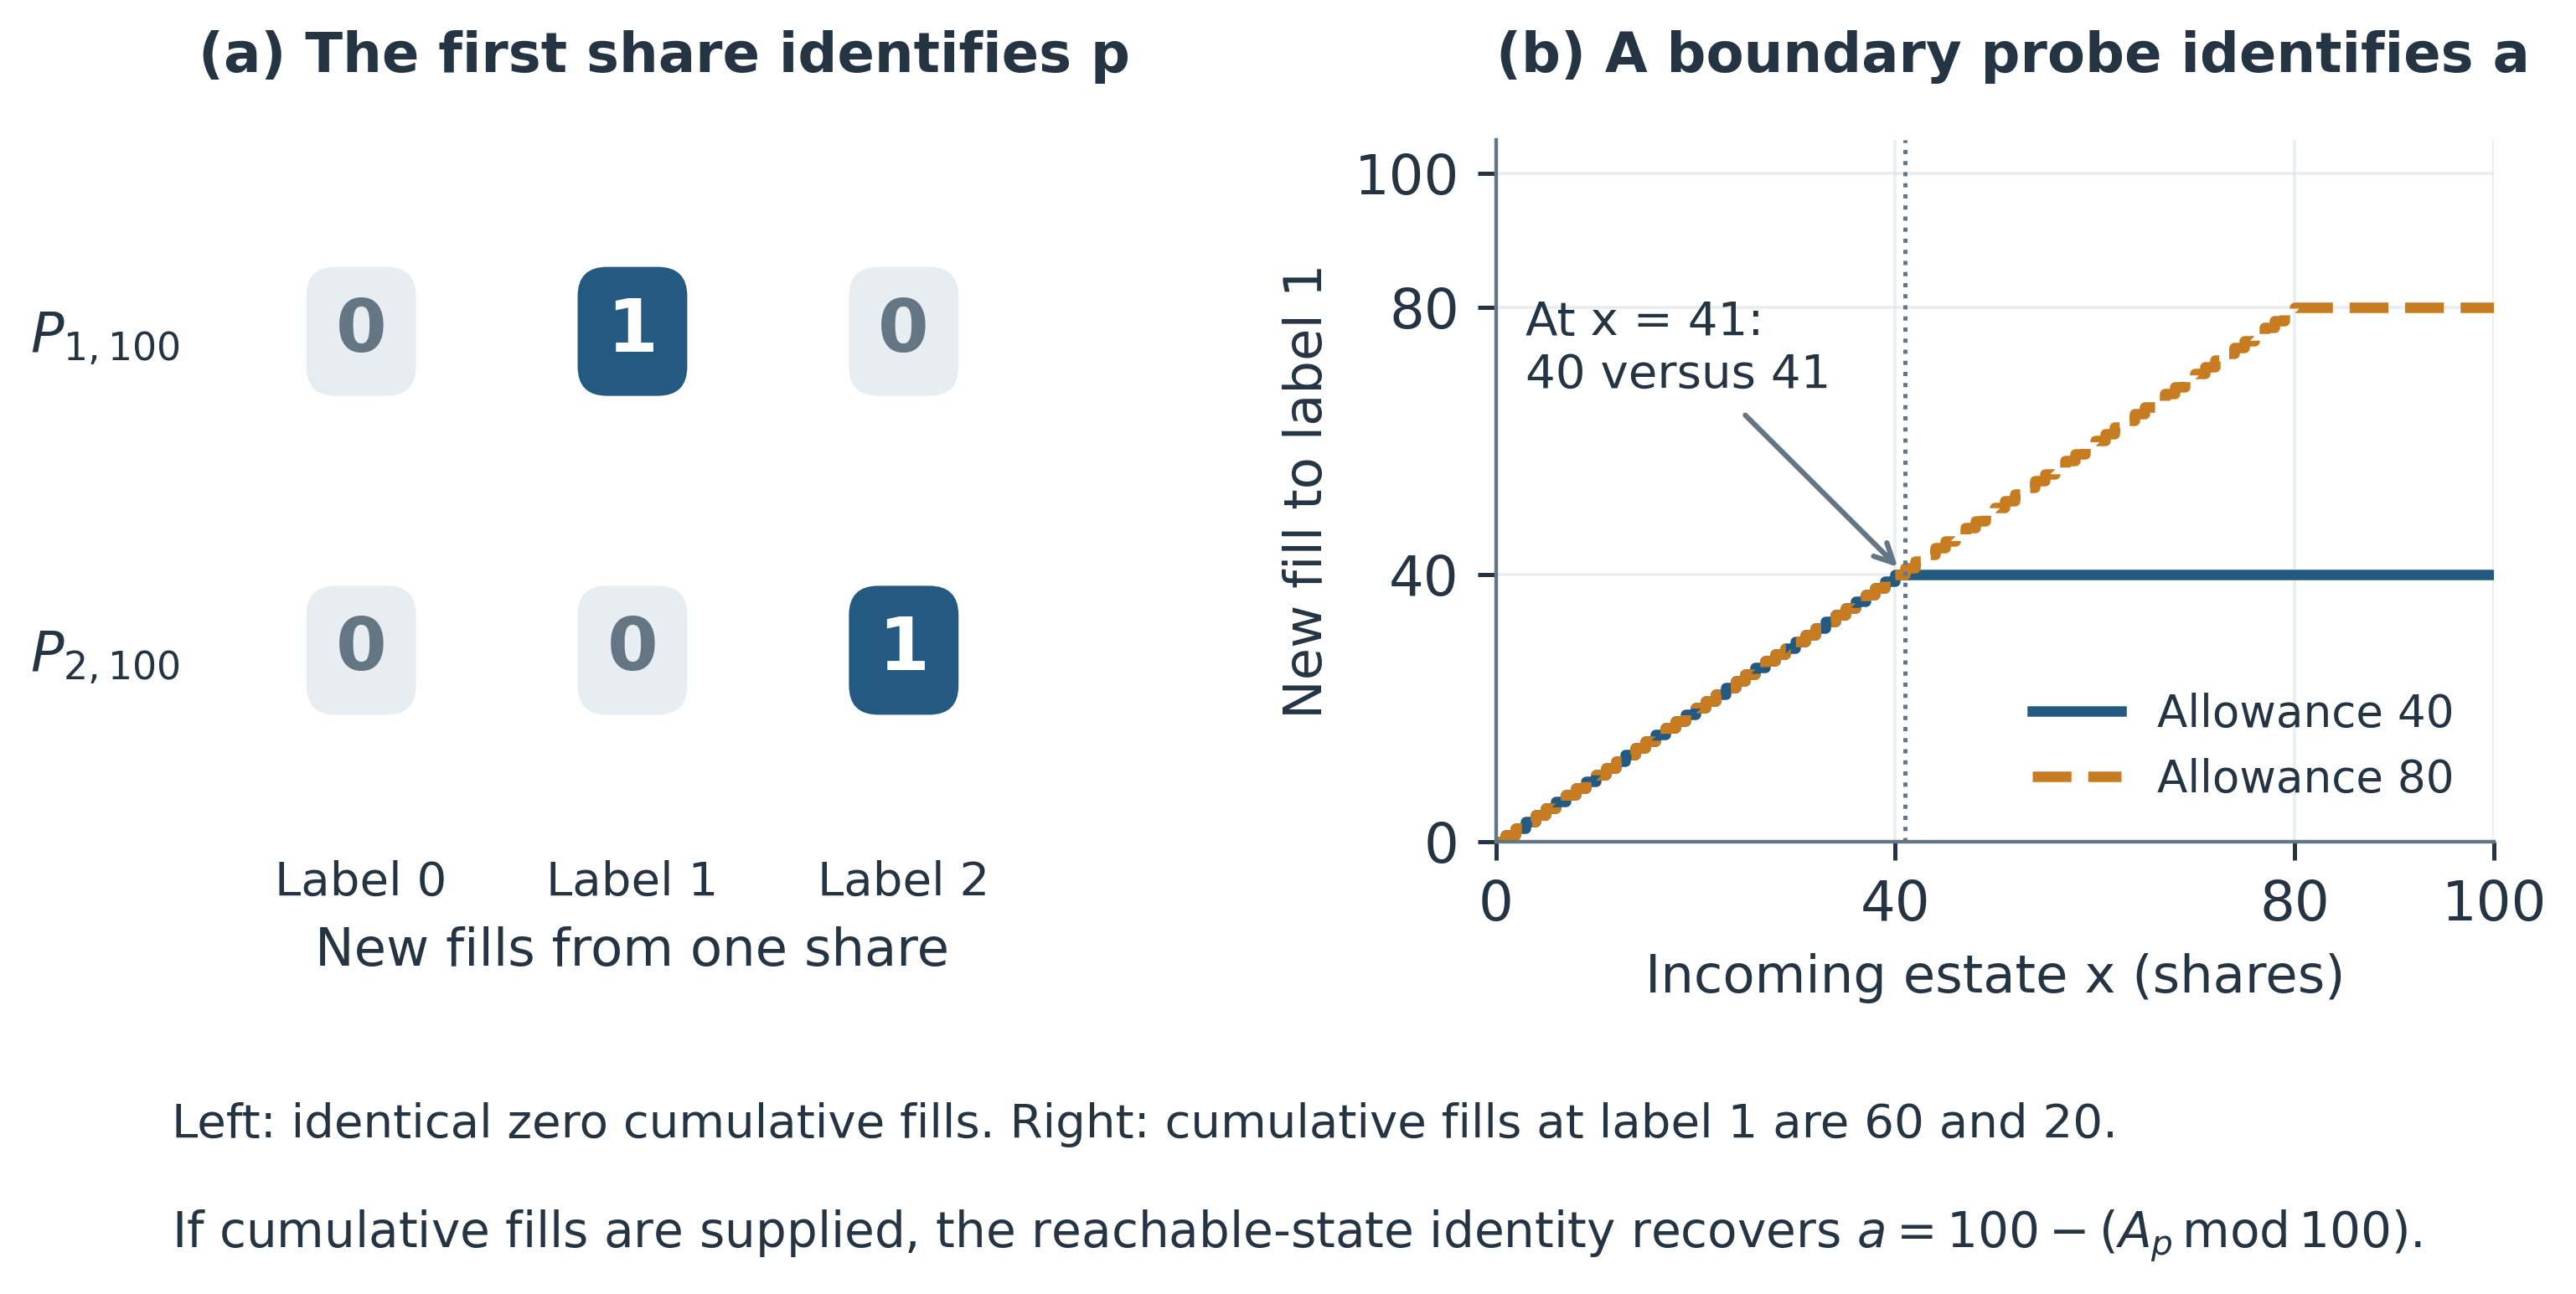
\includegraphics[width=\linewidth]{figures/future_state_probes.png}
\caption{Finite separating probes in the reachable family with $m=3$, $L=100$, and original claims 201. Left: full-allowance phases have identical zero cumulative fills, yet the first share distinguishes pointers 1 and 2. Right: with pointer 1 fixed, the estate $x=41$ distinguishes allowances 40 and 80: new fills are $(0,40,1)$ and $(0,41,0)$. These two phases have different cumulative fills, 60 and 20 at the pointer. When those fills are available, $a=L-(A_p\bmod L)$ recovers the allowance, as in Corollary~\ref{cor:allowance-recovery}.}
\label{fig:probes}
\end{figure}

For comparison, \lean{saturatedOwner} defines an idealized infinite-backlog phase formula with elementary trace-injectivity lemmas. Those lemmas are separate from, and unnecessary for, the finite executable theorem above.

\plain{A public trade tape records executions but does not normally expose the full prior order queue or a participant-aligned allocation vector. Even when an auditor has the stronger aligned record used by these theorems, different hidden queues or pointer states can generate the same fills. The results state exactly what can still be inferred and what cannot be reconstructed from those inputs alone.}

\section{Conformance}\label{sec:conformance}

\begin{corollary}[Decidable, complete, and sequentially composable; \lean{conformsPT}, \lean{conformsPT\_iff}, \lean{conformsPT\_comp}]
The Boolean ``aligned fills equal the engine output'' is decidable and equivalent to ``aligned fills satisfy Axioms~\ref{ax:feas} and~\ref{ax:serial}.''
\end{corollary}
A surveillance rule is, in this foundation, a decidable predicate with a completeness theorem; a flagged allocation record names the axiom it violates. If one aligned fill vector conforms to the original queue and a second conforms to the residual queue, \lean{conformsPT\_comp} proves that their pointwise sum $A\oplus B$ conforms to one execution of the combined quantity. Acceptance is therefore stable when two individually conforming executions are aggregated. \lean{AllocationRecord.lean} implements the one-execution predicate as a program reading lines \texttt{queue;x;fills} and reporting \texttt{OK} or the violated property with the first offending index (\texttt{CAP}, \texttt{CONSERVATION}, \texttt{SERIAL}).

\lean{Conformance.lean} exercises the checker on synthetic allocation records. A fixed-size harness accepts 200/200 engine-generated records and rejects 200/200 single-transfer mutations. A second harness varies incoming size, accepts 200/200 honest records, and rejects 800/800 mutations spanning forward transfer, backward transfer, over-fill, and under-fill. These are deterministic regression tests, not statistical estimates and not an independent implementation of the axioms. The command-line parser rejects any malformed numeric token rather than deleting it. An additional executable regression script checks 12 cases covering valid input, parse rejection, and named length, cap, conservation, and seriality failures. \lean{Collisions.lean} displays explicit distinct queues that generate identical price--time fill vectors; the examples are witnesses, not a population estimate from an unspecified sampling design.

\plain{The checker receives the known or reconstructed queue, incoming quantity, and a privileged queue-aligned fill vector. It either returns \texttt{OK} or names the first violated rule. Passing means the record matches the formal price--time model for those inputs. It does not prove that the supplied queue or order-to-fill alignment is authentic, which is why consolidated trade data by itself is insufficient.}

\section{Rule-by-rule coverage register}\label{sec:rule-register}

This compact register accounts for every analytic market-rule family encoded in the Lean package. The kernel column names the executable abstraction, the guarantee column states only what Lean proves about it, and the boundary column identifies what that theorem leaves outside. The last column points to the corresponding clause-layer record where one exists. Analytic-only entries have no corresponding clause-layer certificate.

\begingroup
\footnotesize
\setlength{\tabcolsep}{2.5pt}
\renewcommand{\arraystretch}{1.00}
\begin{longtable}{@{}>{\raggedright\arraybackslash}p{0.11\textwidth}>{\raggedright\arraybackslash}p{0.19\textwidth}>{\raggedright\arraybackslash}p{0.20\textwidth}>{\raggedright\arraybackslash}p{0.26\textwidth}>{\raggedright\arraybackslash}p{0.17\textwidth}@{}}
\toprule
Family & Kernel & Proved guarantee & Boundary & Clause-layer object \\
\midrule
\endfirsthead
\toprule
Family & Kernel & Proved guarantee & Boundary & Clause-layer object \\
\midrule
\endhead
\bottomrule
\endfoot
Price--time & \lean{priceTime}; \lean{matchAsks} & Unique feasible serial allocation; caps, conservation, monotonicity, and price priority. & Queue construction, modifications, cancellations, hidden priority, self-trade prevention, and venue tie-breaks are inputs or omitted. & \lean{VenueBookState} \\[2pt]
Parity & \lean{wheel}; \lean{discreteCEA}; \lean{runWFull} & Estate rule: feasibility but reset-composition failure. Persistent wheel: one-lot band, reachable composition, allowance recovery, general fiberwise pointer minimality, and exact finite-family quotients. & Global raw-state quotient can collapse at claim boundaries or with one live participant; eligibility, aggregation, label restoration, and within-participant ranking remain inputs \citep{nyse2024parity}. & \lean{VenueBookState}; NYSE ledger ranges \\[2pt]
Hybrid priority & \lean{rule737}; \lean{rule737full} & Setter, displayed, and residual tiers compose and conserve quantity. & Setter eligibility, floor interest, complete rankings, and conditional instructions remain outside the kernel. & \lean{VenueBookState}; \lean{NyseAuctionState} \\[2pt]
Displayed vs hidden & \lean{t3\_only\_after\_t2} & Reachable displayed interest is offered the residual before the modeled hidden tier. & Only two residual pools; not every venue-specific priority category. & \lean{VenueBookState} \\[2pt]
Protected quotes & \lean{protected\_}; \lean{nbo} & The modeled NBO is no worse than any supplied protected offer; manual and sub-round-lot quotes do not set it. & Requires the correct venue-top set, security-specific round lot, accessibility, and data consolidation \citep{sec2005regnms}. & Rule~600 ledger entry; \lean{Rule611State} \\[2pt]
Rule~611 & \lean{tradeThroughBuy}; \lean{sweepThenExecute} & No modeled trade-through at or below NBO; sweeps conserve and satisfy supplied better quotes. & Kernel omits timing, flicker, failures, and most exceptions \citep{sec2008nmsfaq}. & \lean{Rule611State}; \lean{Rule611Exception} \\[2pt]
Self-help & \lean{nboSH} & Removing a venue cannot improve the best remaining offer. & Systems-problem finding, notice, duration, policy, and resumption require evidence. & Rule~611 exception facts \\[2pt]
Rule~610 & \lean{feeCap}; \lean{accessFeeCap610}; \lean{slideBuy} & Fee-spread bound; four dated cap branches; exact legacy dollar-price compatibility; sliding respects limit and avoids a modeled lock. & Fee schedules, rebate tiers, routing economics, and policies are not inferred from price arithmetic. & Dated \lean{FeeProfile610}; September~2026 guard \\[2pt]
Rule~612 & \lean{rule612}; \lean{minimumTick612} & Legacy whole-cent kernel plus no-lock implies a one-cent spread; six dated tick branches; exact legacy predicate compatibility. & The amended profile remains delayed until the cited compliance date; measurement evidence is supplied. & \lean{Rule612State}; schedule and September~2026 guard \\[2pt]
Two clocks & \lean{Ev} & Nonnegative latency, order preservation at equal latency, inversion possibility and bound. & Not SIP sequencing, synchronization, corrections, or feed arbitration \citep{ding2014slow,bartlett2019latency}. & Analytic only; no claimed corpus analogue \\[2pt]
Order types & Midpoint, reserve, discretionary, peg, and post-only kernels & Floored midpoint is in $[\NBB,\NBO)$; exact doubled midpoint is strictly inside; one-refresh conservation, peg monotonicity/no-lock, and non-taking properties. & The floored grid midpoint can equal the NBB at a one-unit spread; not a complete venue order life cycle or interaction model \citep{nasdaq2026equity4}. & \lean{VenueBookState}; Nasdaq type/attribute catalogues \\[2pt]
LULD & \lean{luldBands}; \lean{limitState\_boundary} & Static bands contain the reference and widen with the percentage. & Dynamic reference, tiers, timing, pauses, reopening, dissemination, and procedures are not kernel theorems. & \lean{LuldPlanState} \\[2pt]
Rule~201 & \lean{shortSaleOK} & While the supplied trigger is active, modeled short executions must be above NBB. & Trigger, duration, marking, policies, handling, and exceptions are not derived by this kernel. & \lean{Rule201State}; exception types \\[2pt]
Rule~605 & \lean{effSpread2} & For $px\le\NBO$, the signed $\Z$ kernel is bounded above by quoted spread; it vanishes at an exact midpoint and preserves below-midpoint magnitude. & Not by itself a side-aware reporting system; September and November profiles differ \citep{sec2024rule605,sec2026rule605faq,sec2026rule605order}. & \lean{Rule605Report}; dated profile; exhaustive field types \\[2pt]
Auctions & \lean{crossPrice3}; \lean{dmmFacilitate} & Lexicographic price key; sufficient facilitation clears residual and conserves. & Eligibility, imbalance publication, collars, freezes, reopening, floor procedures, and venue tie-breaks remain external. & \lean{NasdaqCrossState}; \lean{NyseAuctionState} \\[2pt]
State inference & Fingerprint, collision, and wheel-information theorems & Proves general nondegenerate phase separation, exact pointer necessity/sufficiency on common-observation fibers, reachable allowance recovery, and exact separation of $mL$ complete-summary phases. & The $mL$ bound omits side inputs; with aligned cumulative fills supplied, the reachable full-allowance fiber has exactly $m$ pointer states and the allowance is redundant on every reachable live-head state. & Analytic only; reconstruction evidence is external \\[2pt]
Conformance & \lean{conformsPT}; \lean{conformsPT\_comp}; \lean{diagnose} & Boolean equivalence to feasibility and seriality; first failure is named; individually conforming consecutive runs compose. & Price--time needs an authentic queue and order-to-fill alignment; parity additionally needs authenticated pointer state; neither is production-engine or transport certification. & Analytic only; production equivalence is external \\
\end{longtable}
\endgroup

\newcommand{\RegulatoryAppendix}{%
\section{Dated regulatory traceability and inspection}\label{app:clauses}

This section supports exactly three distinct claims: the preceding source proves mathematical deductions, the clause ledger provides compiler-linked traceability into a fixed corpus, and real-world compliance still requires independent legal, evidentiary, and implementation review. The allocation operators and rule-inspection records share one formal development, but the evidence standard does not. The profiles and mappings below make the second claim reviewable without promoting it into either of the other two.

The traceability unit is an expressly cited paragraph, paragraph range, or identified Commission guidance/order item, not necessarily one row per printed subparagraph. A compiler-linked destination ensures that a referenced formal object exists and survives refactoring. It does not establish that the destination faithfully or sufficiently interprets the source.

\subsection{Fixed and dated corpus}

The 58 rows comprise 43 federal and federal-supporting ranges, five LULD Plan ranges, three NYSE ranges, and seven Nasdaq ranges. The federal snapshot is the eCFR text current through September~2, 2026, read with operative-date, guidance, and exemptive-relief materials; NYSE and LULD texts were accessed September~4, 2026, and the Nasdaq catalogue and cited ranges were checked again on September~5, 2026 \citep{ecfr2026regnms,ecfr2026regsho,nyse2026rules,nasdaq2026equity4,luld2026plan}. The corpus is:

\begin{itemize}[leftmargin=*]
  \item three Rule~600(b) rows---general incorporated definitions, paragraph (89)(i)(F) minimum-increment indicator with its June~2026 relief profile, and paragraph (93) round-lot tiers---plus eight Rule~610 ranges, six Rule~611 ranges, seven Rule~612 ranges, nine Rule~201 ranges, and ten Rule~605 rule/guidance/order ranges, so $3+8+6+7+9+10=43$;
  \item five operative LULD Plan ranges grouping definitions and coverage, reference and numerical rules, band and pause states, reopening and halts, and dissemination/policy/overnight duties;
  \item NYSE Rules~7.31(a)--(i), 7.35 general/A/B, and 7.37(a)--(g); and
  \item Nasdaq Rules~4702(a), 4702(b)(1)--(17), 4703(a)--(m), 4752(a)--(d), 4753(a)--(e), 4754(a)--(b), and 4757(a)--(c).
\end{itemize}

These counts describe mapping granularity. They are not a count of every nested sentence, proviso, cross-reference, or provision elsewhere in the Exchange Act, Regulation NMS, Regulation SHO, or the complete venue rulebooks. Completeness is claimed only for finite formal catalogues whose constructors and advertised lists are explicitly compared by Lean.

\subsection{Formalization of non-numerical duties}

A numerical clause is executable. For example, \lean{accessFeeCap610} selects the fee cap from an explicit profile and price; \lean{minimumTick612} selects the increment from profile, price, spread, and new-stock status; and \lean{tenPercentDecline201} evaluates the short-sale trigger.

A legal exception is represented by a finite reason together with the facts that validate it. \lean{Rule611Exception} has one constructor for each Rule~611(b) exception. \lean{ShortExemptReason201} and \lean{ShortExemptFacts201} encode the Rule~201 short-exempt bases and their internal conditions. Whole-record relief is not a bypass switch: \lean{ExemptionAttestation} separately records a grant, coverage of every checked duty, and satisfaction of stated conditions. Partial relief must be represented at the affected duty.

Procedural language such as establishing written policies becomes a named Boolean attestation. That makes the premise visible and machine-checkable, but the Boolean is not evidence. It does not authenticate manuals, notices, surveillance records, market data, or production behavior. Provenance and independent verification remain external.

\subsection{Federal specifications}

\subsubsection{Rule 600 definitions}

General incorporated definitions exclude paragraphs (89)(i)(F) and (93), which have dedicated rows. Paragraph (89)(i)(F) requires an indicator of the applicable minimum pricing increment under Rule~612; it is not the odd-lot-information definition. Its \lean{MinimumIncrementIndicatorProfile600} selects the June~11, 2026 relief regime for the September snapshot. Odd-lot information is defined in paragraph (69), including the best odd-lot additions in (69)(iii), and has a distinct dissemination timetable. The adopted text makes this distinction on printed pages 512--513 of Release No.~34-101070; the indicator's relief is stated on pages 5--6 and 8 of Release No.~34-105656 \citep{sec2024nms,sec2026relief}.

Paragraph (93) has the numerical \lean{roundLotSize600} kernel: 100 shares through $\$250$, 40 through $\$1{,}000$, 10 through $\$10{,}000$, one above that, and 100 for a new NMS stock. The inspected interface \lean{checkedRoundLotSize600} accepts an existing-stock average supplied in normalized cents, represented in the paper's $\$0.0001$ units, and rejects off-grid inputs. It therefore does not silently classify $\$250.0001$: that input returns \lean{none}, whereas $\$250.01$ returns 40. Five tier lemmas and four interface/boundary lemmas verify the numerical behavior. The input's normalization, primary-exchange provenance, and assignment to the March/September evaluation and May/November operative periods remain explicit external duties. The interface does not prescribe a rounding policy for raw averages; paragraph (93) and its operative timetable are on printed pages 513--514 of the adopting release \citep{sec2024nms}.

\subsubsection{Rule 610}

\lean{Rule610State} separately records fair access to an SRO trading facility, equivalent and nondiscriminatory access to a display-only facility, the price-dependent fee cap, fee transparency at execution, lock/cross controls, pattern-or-practice control, and scoped Commission relief. \lean{FeeProfile610} distinguishes the legacy cap used during the September~2026 relief period from the lower amended cap. Four branch theorems prove the dollar and sub-dollar formulas. \lean{rule610Complies} rejects the amended profile for the dated snapshot; \lean{rule610\_amended\_profile\_not\_september2026} proves that guard \citep{sec2024nms,sec2026relief}. The Commission's June~11, 2026 action concerning Rules~611 and 610(e) was a rescission proposal, not a final rescission; the fixed corpus therefore retains both operative specifications and labels the proposal as such \citep{sec2026proposal}.

\subsubsection{Rule 611}

\lean{Rule611State} requires written policies, regular surveillance, prompt remediation, transaction-level protection, ISO reasonable steps, and any scoped relief. \lean{Rule611Exception} exhausts system failure, non-regular-way settlement, single-price auctions, crossed protected markets, incoming ISO, outbound ISO sweep, benchmark trades, the one-second quotation condition, and stopped orders. The stopped-order case additionally requires customer status, order-by-order agreement, and the prescribed price relation. \lean{rule611Complies} rejects a trade-through unless a fully conditioned alternative holds.

\subsubsection{Rule 612}

\lean{Rule612State} records the pricing profile, evaluation and operative periods, primary-listing-exchange measurement, covered price, new-stock status, display, ranking, acceptance, indications of interest, and scoped relief. \lean{operativePeriodFor612} maps January--March measurements to May--October and July--September measurements to November--April. \lean{minimumTick612} encodes both the legacy-relief profile and the delayed amended profile. Six theorems prove the profile/price branches; \lean{rule612\_iff\_minimumTick612\_legacy} proves agreement with the analytic legacy predicate. The September guard prevents the delayed amended profile from being reported as the current decision \citep{sec2026relief}.

\subsubsection{Rule 201}

\lean{restrictionApplies201} derives the ten-percent decline condition, requires listing-market determination and notice, restricts the remainder of that day and the following day, and requires a continuously disseminated NBB. \lean{transactionAllowed201} implements the above-NBB, initially displayed, and short-exempt alternatives. \lean{validShortExempt201} checks ownership/delivery restriction, odd-lot market making, convertible and foreign arbitrage, underwriting cases, riskless-principal sequencing/allocation/records, and VWAP conditions. Policies, surveillance, remediation, SRO conformity, and valid scoped relief complete \lean{rule201Complies}.

\subsubsection{Rule 605}

The amended schema is finite and encoded without ellipses. \lean{OrderType605} has ten covered order classes. \lean{CoreField605}, \lean{ImmediateField605}, \lean{NonmarketableField605}, and \lean{SummaryField605} contain 25, 19, 4, and 12 fields. Five \lean{*605\_complete} theorems prove by exhaustive case analysis that each full-schema list contains every constructor.

The general compliance date for the 2024 Rule~605 amendments was August~1, 2026. SEC Rule~605 FAQ~39, answer A39, states that collection of the five best-available-displayed-price statistics begins November~1, 2026 and that the first reports containing them are due at the end of December~2026; FAQ footnote~2 identifies ten order types per security \citep{sec2026rule605faq}. \lean{Rule605Profile} therefore distinguishes \lean{augustThroughOctober2026} from \lean{november2026AndLater}. The first profile requires 14 immediate fields and the second all 19. Theorems prove both branches and reject the 19-field profile for September. \lean{Rule605Report} also records the treatments in Sections~II.A--II.B of the April~1, 2026 order, Exchange Act Release No.~34-105136 \citep{sec2026rule605order}. \lean{publicationRoute605} uses uniform plan access when an effective joint plan exists and the free, machine-readable website fallback otherwise.

\subsection{Plan and venue specifications}

\subsubsection{Limit Up--Limit Down}

\lean{LuldPlanState} names stock coverage; tier and price classification; rolling reference and change threshold; percentages, late-day doubling, and rounding; execution and quotation bands; limit and straddle states; the pause; reopening and regulatory halts; processor dissemination; participant policies and surveillance; overnight protection; and exemption. \lean{luldPlanComplies} permits no silent omission.

\subsubsection{Nasdaq}

\lean{NasdaqOrderType4702} enumerates the seventeen named types in Rule~4702(b)(1)--(17), including Market On Open and Extended Trading Close. \lean{NasdaqAttribute4703} enumerates the thirteen lettered families in Rule~4703(a)--(m), including Reserve Size, Attribution, and Trade Now. Non-display is treated within the display semantics rather than as an extra lettered paragraph. The exhaustiveness theorems establish completeness of these formal catalogues; they do not establish the order types\textquotesingle{} full behavior. The separate Extended Trading Close procedures in Rule~4755 are outside this ledger. \lean{VenueBookState} covers session eligibility, type semantics, attribute compatibility, Reg NMS and Reg SHO repricing, timestamp behavior, priority, routing, data and fallback sources, locks, self-help, cancellation, and re-entry. \lean{NasdaqCrossState} covers definitions, eligible interest, imbalance data and schedules, price hierarchy, collars, allocation priority, uniform price, official-price dissemination, LULD/hybrid variants, and contingencies.

\subsubsection{NYSE}

The shared book-state record covers Rule~7.31 order/modifier behavior and Rule~7.37 execution, allocation, routing, market data, lock/cross, and self-help duties; \lean{rule737full} and \lean{matchNYSE} are the proved allocation kernels in the foundations paper. \lean{NyseAuctionState} represents Rule~7.35 general, Core Open/Trading Halt, and DMM-facilitated Closing Auction families, including responsibilities, eligibility, entry/modification/cancellation windows, imbalance publication, reference prices, collars/freezes, price determination, priority, facilitation, reopening, and contingencies.

\subsection{Ledger audit and exact force}

The 58-entry \lean{clauseCorpus} maps each identified source unit to a \lean{FormalDestination} and classifies it as a definition, numerical rule, state transition, exception, procedure, or disclosure. A destination stores an actual Lean value, function, projection, or tuple; deleting or renaming the referenced object breaks elaboration.

\begin{auditlemma}[Fixed-corpus checks]
\raggedright
The declarations \lean{clause\_corpus\_has\_58\_entries}, \lean{clause\_corpus\_family\_counts}, \lean{clause\_corpus\_citations\_unique}, and \lean{clause\_corpus\_traceability\_complete} verify, respectively, the total count, the advertised $43+5+3+7$ partition, unique citations, and that every row has readable labels and a compiler-linked destination. They are list-length and elaboration audits, not substantive legal theorems.
\end{auditlemma}

Generated ranges are not deemed complete merely because they have a destination. Rule~605 fields, Rule~611 exceptions, Rule~201 bases, Nasdaq order types, and Nasdaq attributes are finite inductive types compared with exhaustive lists. These audit lemmas do not prove faithful interpretation, sufficient grouping, evidentiary truth, implementation equivalence, or venue compliance.

\subsection{Inspection contract}

\begin{longtable}{@{}>{\raggedright\arraybackslash}p{0.24\textwidth}>{\raggedright\arraybackslash}p{0.32\textwidth}>{\raggedright\arraybackslash}p{0.36\textwidth}@{}}
\toprule
Layer & Machine-checked result & Independent review still required \\
\midrule
\endfirsthead
\toprule
Layer & Machine-checked result & Independent review still required \\
\midrule
\endhead
\bottomrule
\endfoot
Numerical profile & Exact branch result for supplied date/profile inputs & Correct operative law, date, security class, and source facts \\[3pt]
Finite catalogue & Every formal constructor appears in the advertised list & Whether the constructors faithfully partition the controlling text \\[3pt]
Exception & Enumerated reason satisfies encoded internal conditions & Evidence for those facts and legal availability of the exception \\[3pt]
Attestation & Required Boolean fields and scoped-relief conditions are present & Provenance, authenticity, sufficiency, and reviewer judgment \\[3pt]
Clause ledger & 58 unique rows have elaborated destinations and labels & Completeness outside the fixed corpus and semantic quality of each mapping \\
\end{longtable}

}

\section{Regulatory traceability: audit contract}\label{sec:clauses}\label{sec:companion}

This layer supports exactly three claims: the preceding source proves mathematical deductions, a compiler-linked ledger provides traceability into a fixed legal and venue corpus, and real-world compliance still requires independent legal, evidentiary, and implementation review. The proof standards are deliberately different. Appendix~\ref{app:clauses} contains the detailed profiles, source ranges, record types, and pinpoints.

The compiled corpus has 58 rows: 43 federal and federal-supporting ranges, five LULD Plan ranges, three NYSE ranges, and seven Nasdaq ranges. Each row has a unique citation, a readable label, and an elaborated Lean destination. Separate exhaustive-list checks cover the formal Rule~605 fields, Rule~611 exceptions, Rule~201 bases, Nasdaq order types, and Nasdaq attributes. These are audit lemmas about a finite encoding, not theorems that the encoding is a complete or correct legal interpretation.

The federal profiles use primary SEC materials available as of September~5, 2026. Release No.~34-105656 grants the stated relief for Rules~600(b)(89)(i)(F), 610(c), and 612 until the first business day of November~2027; Release No.~34-105655 remains expressly labelled a proposed rescission of Rules~611 and 610(e); Rule~605 FAQ~39 gives the November~1 collection date and end-of-December reporting date; its footnote~2 states ten order types per security; and Release No.~34-105136 is the April~1 Rule~605 exemptive order \citep{sec2026relief,sec2026proposal,sec2026rule605faq,sec2026rule605order}.

\begin{center}
\small
\begin{tabular}{@{}>{\raggedright\arraybackslash}p{0.22\textwidth}>{\raggedright\arraybackslash}p{0.31\textwidth}>{\raggedright\arraybackslash}p{0.37\textwidth}@{}}
\toprule
Layer & Machine-checked result & Independent review still required \\
\midrule
Numerical profile & Exact branch result for supplied inputs & Operative law, date, security class, normalization, and source facts \\[3pt]
Finite catalogue or ledger & Every constructor or fixed row appears once with an elaborated destination & Completeness of the corpus and faithful interpretation of each source \\[3pt]
Exception or attestation & Encoded conditions and required Boolean fields are present & Evidence, provenance, authenticity, legal availability, and implementation behavior \\
\bottomrule
\end{tabular}
\end{center}

The ledger is therefore an inspection artifact attached to the mathematical paper, not evidence that any venue or broker-dealer complies with the mapped provisions.

\section{Scope and limitations}\label{sec:scope}

\paragraph{Decided.} The formal statements attached to the named Lean declarations: three integer allocation operators and their proved algebraic properties; the large-lot wheel-pass endpoint; price--time uniqueness; balance and an explicit run-dependent water level for the pass-based wheel; feasibility of an estate-indexed unit-increment rule and failure of its reset version to compose; one-lot balance and canonical stream composition for the same persistent pointer wheel, with no allowance premise on reachable states; impossibility of parity conformance from queue and aligned fills without pointer evidence; general nondegenerate pointer--allowance separation; exact fiberwise pointer necessity and sufficiency under a common authenticated observation; exact future equivalence, reachability, and the $mL$ complete-summary lower bound for the finite phase family; the exact $m$ pointer bound on the reachable full-allowance common-observation fiber; allowance recovery from cumulative allocation on every reachable live-head state; relabeling equivariance; signed effective-spread arithmetic; cross-market, order-type, auction, observability, and strategic kernels; and price--time conformance equivalence and sequential composition. Section~\ref{sec:clauses} states the distinct fixed-corpus audit results. All 362 theorem declarations are kernel-checked, and the numerical worked examples are decided by evaluation. Fixed-length bit bounds are elementary deductions from the checked injectivity results. Corollary~\ref{thm:continuum} is a conventional real-analysis consequence of the machine-checked finite approximation bound; it is not represented as a separate Lean declaration.

\paragraph{Not decided.} Correctness of a legal interpretation beyond the stated formal mapping; truth, sufficiency, provenance, or authenticity of attestations and underlying evidence; behavioral equivalence between these specifications and a production exchange system; compliance by any real entity; provisions outside the stated fixed corpus; a global minimal quotient of every raw \lean{WState} including claim-boundary and one-live-participant degeneracies; a characterization of all banded stream-consistent mechanisms; reconstruction of an order-level queue or participant alignment from consolidated data; empirical validity on exchange data; composition of the stateless reset estate rule (which is formally refuted); or continuous mixed-strategy equilibria. The executable price--time checker requires an authenticated or reconstructed order-level queue and queue-to-fill alignment and is exercised here only on synthetic inputs.

\paragraph{Security universe.} The operator theorems do not depend on issuer capitalization or index membership. They therefore cover small-cap securities and Russell~3000 constituents whenever the stated queue, lot-size, venue, and state assumptions hold. The paper does not model index construction, constituent selection, capitalization, liquidity, or empirical performance.

\section{Conclusion}\label{sec:programme}

Persistent wheel state restores split-versus-combined consistency lost under reset rotation. Future-fill probes establish pointer necessity on common-observation families, while the reachable phase invariant recovers unused allowance from aligned cumulative fills. These results connect executable allocation semantics to conformance and identifiability. Strategic consequences require additional behavioral assumptions; institutional application requires independent review of rule mappings, evidence, and implementation equivalence.

\appendix
\section{The proof system}
Lean~4.22.0, core library only, as a Lake package with no dependencies. The compiler identifies commit \texttt{ba2cbbf09d4978f416e0ebd1fceeebc2c4138c05} (Release). Modules in build order: \lean{Rule737} (operators, large-lot endpoint, conservation, book share, worked allocation), \lean{Markets} (three tiers, observability, cross, tick and protection, two clocks, routing), \lean{Balance} (state-form wheel, explicit water level, balance theorem, two-level clearing key, fee cap), \lean{Rulebook} (uniqueness, conformance, serial ladder, consolidation, sweep, sliding), \lean{Orders} (order types, self-help, exact doubled midpoint, three-level clearing key, facilitation), \lean{Strategic} (contests, dilution, routing), \lean{SetterRace} (all-pay race), \lean{Closure} (wheel agreement, $\varepsilon$-equilibrium), \lean{Conformance} and \lean{Collisions} (synthetic allocation records and collision witnesses), \lean{Algebra} (operator monoid, conservation closure, impossibility, ladder uniqueness), \lean{MoreRules} (completeness, estate completion/reset obstruction, signed execution-quality kernel, bands, close eligibility, post-only), \lean{PathIndependence} (composition boundaries, canonical fuel, reachable phase invariant, idealized owner trace, pointer-relative balance), \lean{WheelInformation} (general phase separation, fiberwise pointer minimality, finite-family reachability and exact quotients, reachable allowance recovery, relabeling equivariance, book-share counterexample), \lean{ClauseComplete} (dated profiles, compatibility lemmas, 58-row ledger, finite schemas, exceptions, attestations, and checklist predicates), \lean{Check} (exhaustive theorem-axiom audit), and \lean{AllocationRecord} (executable checker). All 362 theorem declarations depend on at most \lean{propext}, \lean{Quot.sound}, and \lean{Classical.choice}; worked examples depend on none.

\paragraph{Classical-choice audit.}
No source definition is marked \lean{noncomputable}, and the source contains no call to \lean{Classical.choose}. The executable \lean{AllocationRecord} path uses \lean{parseNats}, \lean{firstDiff}, \lean{diagnose}, \lean{conformsPT}, and \lean{priceTime}; none has an audited theorem dependency because definitions are evaluated rather than proved. Exactly 48 theorem proof terms include \lean{Classical.choice}:

\begingroup\small\raggedright
\lean{wheelOp\_conserves}, \lean{wheelOpFull\_conserves}, \lean{rule737Op\_conserves}, \lean{ladder\_unique}, \lean{wheelS\_within\_L}, \lean{wheelS\_within\_L\_explicit}, \lean{wheelS\_eq\_wheel}, \lean{wheel\_balanced}, \lean{wheelS\_state\_eq}, \lean{wheel\_within\_L}, \lean{uniform\_eps}, \lean{uniform\_eps\_relative}, \lean{priceTime\_tail\_invisible}, \lean{priceTime\_boundary\_invisible}, \lean{rule737full\_sum}, \lean{t3\_only\_after\_t2}, \lean{hidden\_depth\_lower\_bound}, \lean{supplyAt\_zero\_of\_none}, \lean{matched\_dominated\_by\_ask\_price}, \lean{crossPrice\_global}, \lean{wheel\_exhausts}, \lean{discreteCEA\_feasible}, \lean{matchNYSE\_conserve}, \lean{nyse\_price\_priority}, \lean{effSpread2\_neg\_iff}, \lean{midpoint\_inside}, \lean{midpoint2\_strict\_inside}, \lean{mpl\_no\_trade\_through}, \lean{zip\_zero\_add}, \lean{priceTime\_comp}, \lean{conformsPT\_comp}, \lean{saturated\_future\_equiv\_iff}, \lean{saturated\_future\_sufficient\_injective}, \lean{runW\_stops\_of\_tot\_lt\_fuel}, \lean{runWFull\_stopped}, \lean{runWFull\_allocates\_first}, \lean{runWFull\_comp}, \lean{runWFull\_comp\_reachable}, \lean{wheel\_sum}, \lean{rule737\_sum}, \lean{nextWFill\_crosses\_allowance}, \lean{validWheelPhase\_probe\_equiv\_implies}, \lean{wheelFiberSufficient\_pointer\_injective}, \lean{phaseState\_allowance\_probe}, \lean{phaseState\_probe\_equiv\_iff}, \lean{phaseState\_future\_equiv\_iff}, \lean{wheelPhaseSufficient\_injective}, \lean{phaseState\_full\_summary\_injective}.\par
\endgroup
This proof dependency does not make the definitions non-executable.

\subsection{Load-bearing theorem contracts}
The table records the hypotheses that must travel with the headline results. It is a reading aid, not a substitute for the elaborated declarations.

\begingroup
\footnotesize
\setlength{\tabcolsep}{3pt}
\renewcommand{\arraystretch}{1.12}
\begin{longtable}{@{}>{\raggedright\arraybackslash}p{0.24\textwidth}>{\raggedright\arraybackslash}p{0.28\textwidth}>{\raggedright\arraybackslash}p{0.40\textwidth}@{}}
\toprule
Declaration & Required hypotheses / domain & Exact force of conclusion \\
\midrule
\endfirsthead
\toprule
Declaration & Required hypotheses / domain & Exact force of conclusion \\
\midrule
\endhead
\bottomrule
\endfoot
\lean{serial\_unique} & Lists $Q,A$, quantity $x$; \lean{Feasible Q A x}; \lean{Serial A Q}. & $A=\lean{priceTime}\,Q\,x$. It does not authenticate $Q$ or identify venue-specific queue construction. \\[2pt]
\lean{runW\_band} & Natural $L,n,x$; participant-labelled records $R$; $0<L$; state initialized by \lean{initW}. & Some $w$ makes the returned participant state satisfy \lean{Band L w}. It is fuel-bounded and says nothing about eligibility inputs. \\[2pt]
\lean{runW\_comp} & First run has zero leftover; second result satisfies \lean{Stopped}; combined run receives fuel $n_1+n_2$. & Split and combined runs return exactly the same rotated state and leftover. No claim without the completion and termination premises. \\[2pt]
\lean{runWFull\_comp} & $0<L$; positive current allowance; first estate $x\le\lean{totW}(st.S)$; canonical fuel $\lean{totW}(st.S)+1$. & For every $y$, combined and split canonical runs are exactly equal. Completion, stopping, and fuel are derived rather than supplied. \\[2pt]
\lean{runWFull\_comp\_reachable} & State returned by \lean{runW} from \lean{initW}; $0<L$; first estate $x\le\lean{totW}(st.S)$. & The same exact split/combined equality, with current-allowance positivity derived from reachability. \\[2pt]
\lean{future\_sufficient\_summary\_requires\_pointer\_information} & Arbitrary summary codomain; a predictor correct for every four-party state and next quantity from canonical queue, cumulative fills, summary, and quantity. & The summary must distinguish \lean{pointerA} from \lean{pointerC}. This is a witness-level information lower bound, not global minimality of \lean{WState}. \\[2pt]
\lean{validWheelPhase\_probe\_equiv\_implies} & Two states with distinct live head/successor labels, allowances in $[1,L]$, and every remaining claim above $L$. & Equality of all participant-labelled probes through $L$ forces equal pointer labels and allowances; other state components are not thereby identified. \\[2pt]
\lean{wheelFiberSufficient\_pointer\_injective}; \lean{wheelPointerCode\_fiber\_sufficient} & Any one-state-per-pointer nondegenerate family; $L>0$; an authenticated observation common across that family; one decoder correct for every indexed state, estate, and label. & Every future-sufficient summary is injective in the pointer, and the head label is sufficient for the fixed family. This is exact fiberwise minimality, not a global quotient of arbitrary raw states. \\[2pt]
\lean{phaseState\_future\_equiv\_iff}; \lean{wheelPhaseSufficient\_injective} & Reachable family $P_{p,a}$; $m\ge2$; $p<m$; $1\le a\le L$; complete summary with no separate queue/fill input. & Actual \lean{runWFull} probes of size at most $L$ separate every phase. The pair is sufficient. Counting yields $mL$ classes and the binary bit bound. \\[2pt]
\lean{phaseState\_full\_summary\_injective}; \lean{phaseState\_full\_pointer\_sufficient} & Reachable fresh-lot states $P_{p,L}$; $m\ge2$; $L>0$; aligned cumulative-allocation observation supplied. & The common zero observation still requires $m$ distinct summary values, and the pointer supplies exactly $m$. The bit bound is the elementary encoding corollary. \\[2pt]
\lean{runW\_allowance\_phase} & State returned by \lean{runW} from \lean{initW}; $L>0$; returned state has a live head with cumulative allocation $A_p$. & Its allowance is $L-(A_p\bmod L)$. The cycle-phase equation and allowance positivity are derived rather than supplied. \\[2pt]
\lean{runWFull\_relabel} & Relabel every identifier consistently; preserve the ordered records and allowance. & The canonical returned state is relabeled and the leftover unchanged. For bijective labels this preserves a valid participant set. \\[2pt]
\lean{checkedRoundLotSize600\_off\_grid} & Existing stock; price input in $\$0.0001$ units; input not divisible by 100. & Returns no tier. Normalization and the legal evaluation/operative period require independent evidence. \\[2pt]
\lean{discreteCEA\_feasible}; \lean{discreteCEA\_reset\_not\_composable} & Any natural claims and estate for feasibility; fixed claims $(10,10)$ for the counterexample. & The unit rule completes every integer estate, but deterministic rotation reset violates composition: two one-unit estates differ from one two-unit estate. \\[2pt]
\lean{waterFill\_two\_equal\_no\_single\_share} & Any natural water level $s$; fixed claims $(10,10)$. & Benchmark award sum is not 1. Therefore natural water levels do not parameterize every integer estate. \\[2pt]
\lean{conformsPT\_iff} & Supplied queue $Q$, aligned fill vector $A$, and quantity $x$. & Boolean acceptance iff $A$ is feasible and serial relative to those supplied inputs. No authenticity or public-tape reconstruction guarantee. \\[2pt]
\lean{midpoint2\_strict\_inside} & Natural $nbb<nbo$. & $2nbb<nbb+nbo<2nbo$ in doubled units. The integer-grid \lean{midpoint} theorem is only half-open. \\[2pt]
\lean{clause\_corpus\_has\_58\_entries} & The fixed compiled \lean{clauseCorpus}. & Its list length is 58; this is an audit lemma, not semantic or legal completeness. \\
\end{longtable}
\endgroup

\subsection{Paper and source availability}
The paper's DOI is \href{https://doi.org/10.5281/zenodo.22343804}{10.5281/zenodo.22343804}.

The Lean source code, proof scripts, and reproducible build instructions will be made publicly available shortly at \url{https://github.com/MiquelNoguerAlonso/Formal-Verification}. The release will include the LaTeX sources, the five PNG figures, their numerical data and generation scripts, a deterministic build script, and a SHA-256 manifest for the distributed files. The figure data are exported from the executable Lean definitions and checked by an independent Python calculation before rendering at 450 dpi. The figures visualize finite worked examples; they are not empirical estimates. No empirical dataset is used.

\clearpage
\RegulatoryAppendix

\section{Compiler-checkable source excerpt}
The definitions below are an ASCII transcription of the corresponding Lean source; \lean{Prod} denotes an ordered pair. The final \lean{\#check} commands resolve thirteen declarations, including the general phase-separation, fiberwise pointer-minimality, and reachable allowance theorems.
\begin{lstlisting}[basicstyle=\ttfamily\scriptsize]
import Rulebook
import Balance
import PathIndependence
import WheelInformation
import Strategic
namespace PaperExcerpt

def give (L r x : Nat) : Nat := min L (min r x)

def wheelRound (L : Nat) : List Nat -> Nat -> Prod (List Nat) Nat
  | [], x => ([], x)
  | r :: R, x =>
      let g := give L r x
      let p := wheelRound L R (x - g)
      (g :: p.1, p.2)

def wheel (L : Nat) : Nat -> List Nat -> Nat -> Prod (List Nat) Nat
  | 0, R, x => (R.map (fun _ => 0), x)
  | n + 1, R, x =>
      if x = 0 then (R.map (fun _ => 0), x)
      else
        let p := wheelRound L R x
        let R' := List.zipWith (fun r g => r - g) R p.1
        let q := wheel L n R' p.2
        (List.zipWith (fun a b => a + b) p.1 q.1, q.2)

def priceTime : List Nat -> Nat -> List Nat
  | [], _ => []
  | q :: Q, x => min q x :: priceTime Q (x - min q x)

#check @Rule737.serial_unique
#check @Rule737.wheelS_band
#check @Rule737.runW_band
#check @Rule737.runWFull_comp_reachable
#check @Rule737.tullock_best_response
#check @Rule737.validWheelPhase_probe_equiv_implies
#check @Rule737.wheelFiberSufficient_pointer_injective
#check @Rule737.phaseState_future_equiv_iff
#check @Rule737.phaseState_reachable
#check @Rule737.wheelPhaseCode_sufficient
#check @Rule737.phaseState_full_summary_injective
#check @Rule737.runW_allowance_phase
#check @Rule737.runWFull_relabel
end PaperExcerpt
\end{lstlisting}

\StrategicAppendix

\footnotesize
\setlength{\bibsep}{2pt}
\bibliographystyle{plainnat}
\bibliography{refs}
\end{document}
